%File: formatting-instructions-latex-2024.tex
%release 2024.0
\documentclass[letterpaper]{article} % DO NOT CHANGE THIS
\usepackage{aaai24}  % DO NOT CHANGE THIS
\usepackage{times}  % DO NOT CHANGE THIS
\usepackage{helvet}  % DO NOT CHANGE THIS
\usepackage{courier}  % DO NOT CHANGE THIS
\usepackage[hyphens]{url}  % DO NOT CHANGE THIS
\usepackage{graphicx} % DO NOT CHANGE THIS
\urlstyle{rm} % DO NOT CHANGE THIS
\def\UrlFont{\rm}  % DO NOT CHANGE THIS
\usepackage{natbib}  % DO NOT CHANGE THIS AND DO NOT ADD ANY OPTIONS TO IT
\usepackage{caption} % DO NOT CHANGE THIS AND DO NOT ADD ANY OPTIONS TO IT
\frenchspacing  % DO NOT CHANGE THIS
\setlength{\pdfpagewidth}{8.5in}  % DO NOT CHANGE THIS
\setlength{\pdfpageheight}{11in}  % DO NOT CHANGE THIS
%
% These are recommended to typeset algorithms but not required. See the subsubsection on algorithms. Remove them if you don't have algorithms in your paper.
\usepackage{algorithm}
\usepackage{algorithmic}

\usepackage{amsmath}
\usepackage{amsfonts}
\DeclareMathOperator*{\argmax}{arg\,max}
\DeclareMathOperator*{\argmin}{arg\,min}

\usepackage{amsthm}
\newtheorem{definition}{Definition}[section]

\usepackage{xcolor}
\usepackage{colortbl}
\renewcommand{\algorithmicrequire}{\textbf{Input:}}
\renewcommand{\algorithmicensure}{\textbf{Output:}}

%
% These are are recommended to typeset listings but not required. See the subsubsection on listing. Remove this block if you don't have listings in your paper.
\usepackage{newfloat}
\usepackage{listings}
\DeclareCaptionStyle{ruled}{labelfont=normalfont,labelsep=colon,strut=off} % DO NOT CHANGE THIS
\lstset{%
	basicstyle={\footnotesize\ttfamily},% footnotesize acceptable for monospace
	numbers=left,numberstyle=\footnotesize,xleftmargin=2em,% show line numbers, remove this entire line if you don't want the numbers.
	aboveskip=0pt,belowskip=0pt,%
	showstringspaces=false,tabsize=2,breaklines=true}
\floatstyle{ruled}
\newfloat{listing}{tb}{lst}{}
\floatname{listing}{Listing}
%
% Keep the \pdfinfo as shown here. There's no need
% for you to add the /Title and /Author tags.

% DISALLOWED PACKAGES
% \usepackage{authblk} -- This package is specifically forbidden
% \usepackage{balance} -- This package is specifically forbidden
% \usepackage{color (if used in text)
% \usepackage{CJK} -- This package is specifically forbidden
% \usepackage{float} -- This package is specifically forbidden
% \usepackage{flushend} -- This package is specifically forbidden
% \usepackage{fontenc} -- This package is specifically forbidden
% \usepackage{fullpage} -- This package is specifically forbidden
% \usepackage{geometry} -- This package is specifically forbidden
% \usepackage{grffile} -- This package is specifically forbidden
% \usepackage{hyperref} -- This package is specifically forbidden
% \usepackage{navigator} -- This package is specifically forbidden
% (or any other package that embeds links such as navigator or hyperref)
% \indentfirst} -- This package is specifically forbidden
% \layout} -- This package is specifically forbidden
% \multicol} -- This package is specifically forbidden
% \nameref} -- This package is specifically forbidden
% \usepackage{savetrees} -- This package is specifically forbidden
% \usepackage{setspace} -- This package is specifically forbidden
% \usepackage{stfloats} -- This package is specifically forbidden
% \usepackage{tabu} -- This package is specifically forbidden
% \usepackage{titlesec} -- This package is specifically forbidden
% \usepackage{tocbibind} -- This package is specifically forbidden
% \usepackage{ulem} -- This package is specifically forbidden
% \usepackage{wrapfig} -- This package is specifically forbidden
% DISALLOWED COMMANDS
% \nocopyright -- Your paper will not be published if you use this command
% \addtolength -- This command may not be used
% \balance -- This command may not be used
% \baselinestretch -- Your paper will not be published if you use this command
% \clearpage -- No page breaks of any kind may be used for the final version of your paper
% \columnsep -- This command may not be used
% % \newpage -- No page breaks of any kind may be used for the final version of your paper
% \pagebreak -- No page breaks of any kind may be used for the final version of your paperr
% \pagestyle -- This command may not be used
% \tiny -- This is not an acceptable font size.
% \vspace{- -- No negative value may be used in proximity of a caption, figure, table, section, subsection, subsubsection, or reference
% \vskip{- -- No negative value may be used to alter spacing above or below a caption, figure, table, section, subsection, subsubsection, or reference

\usepackage{bm}
\usepackage{array}

\usepackage{booktabs}
\usepackage{multirow}
\usepackage{subcaption}
\usepackage{xcolor}
\usepackage{colortbl}
\usepackage{pifont}
\renewcommand{\algorithmicrequire}{\textbf{Input:}}
\renewcommand{\algorithmicensure}{\textbf{Output:}}
\newcommand{\colorann}[3]{\textcolor{#1}{${}^{#2}[$#3$]$}}
\newcommand{\zt}[1]{\colorann{red}{zt}{#1}}

\setcounter{secnumdepth}{0} %May be changed to 1 or 2 if section numbers are desired.

% The file aaai24.sty is the style file for AAAI Press
% proceedings, working notes, and technical reports.
%

% Title

% Your title must be in mixed case, not sentence case.
% That means all verbs (including short verbs like be, is, using,and go),
% nouns, adverbs, adjectives should be capitalized, including both words in hyphenated terms, while
% articles, conjunctions, and prepositions are lower case unless they
% directly follow a colon or long dash
\title{Sparsity-Guided Holistic Explanation for LLMs with\\ Interpretable Inference-Time Intervention}
\author{
    %Authors
    % All authors must be in the same font size and format.
   Zhen Tan\textsuperscript{\rm 1}, Tianlong Chen\textsuperscript{\rm 2}, Zhenyu Zhang\textsuperscript{\rm 3}, Huan Liu\textsuperscript{\rm 1}
}
\affiliations{
    %Afiliations
    \textsuperscript{\rm 1}Arizona State University\\
    \textsuperscript{\rm 2}University of North Carolina at Chapel Hill\\
    \textsuperscript{\rm 3}University of Texas at Austin
    \\\{ztan36,huanliu\}@asu.edu, tianlong@cs.unc.edu, zhenyu.zhang@utexas.edu
    % Association for the Advancement of Artificial Intelligence\\
    % % If you have multiple authors and multiple affiliations
    % % use superscripts in text and roman font to identify them.
    % % For example,

    % % Sunil Issar\textsuperscript{\rm 2},
    % % J. Scott Penberthy\textsuperscript{\rm 3},
    % % George Ferguson\textsuperscript{\rm 4},
    % % Hans Guesgen\textsuperscript{\rm 5}
    % % Note that the comma should be placed after the superscript

    % 1900 Embarcadero Road, Suite 101\\
    % Palo Alto, California 94303-3310 USA\\
    % % email address must be in roman text type, not monospace or sans serif
    % proceedings-questions@aaai.org
%
% See more examples next
}

%Example, Single Author, ->> remove \iffalse,\fi and place them surrounding AAAI title to use it
\iffalse
\title{My Publication Title --- Single Author}
\author {
    Author Name
}
\affiliations{
    Affiliation\\
    Affiliation Line 2\\
    name@example.com
}
\fi

\iffalse
%Example, Multiple Authors, ->> remove \iffalse,\fi and place them surrounding AAAI title to use it
\title{My Publication Title --- Multiple Authors}
\author {
    % Authors
    First Author Name\textsuperscript{\rm 1,\rm 2},
    Second Author Name\textsuperscript{\rm 2},
    Third Author Name\textsuperscript{\rm 1}
}
\affiliations {
    % Affiliations
    \textsuperscript{\rm 1}Affiliation 1\\
    \textsuperscript{\rm 2}Affiliation 2\\
    firstAuthor@affiliation1.com, secondAuthor@affilation2.com, thirdAuthor@affiliation1.com
}
\fi


% REMOVE THIS: bibentry
% This is only needed to show inline citations in the guidelines document. You should not need it and can safely delete it.
% \usepackage{bibentry}
% END REMOVE bibentry

\begin{document}

\maketitle

\begin{abstract}
% Large Language Models (LLMs) have significantly advanced various natural language processing tasks. However, their ``black-box'' nature creates interpretability challenges, which poses difficulties for responsible usage. Earlier methods to enhance their interpretability, such as visualizing attention weights in transformer layers, extracting essential subnetworks, and concept-based analysis, can only offer either local or global explanations in one dimension. These unidimensional interpretations often lack clarity, comprehensibility, and intuitiveness. In this study, we propose a holistic approach for interpreting LLMs. Uniquely, our method, achieved through rigorous concept-induced sparsity mining, targets three levels of interpretation simultaneously within a single framework, SparseCBM. This approach enables interpretation at the input, subnetwork, and concept levels concurrently. Using real-world datasets for practical evaluations, we demonstrate that our methodology offers a holistic understanding of LLM behavior, and carries distinct advantages in pinpointing and rectifying model errors.

% Large Language Models (LLMs) have ushered in remarkable advancements across a spectrum of natural language processing tasks. Nevertheless, their enigmatic ``black-box'' nature presents a formidable hurdle to attain interpretability, impeding responsible deployment. Former strategies aimed at bolstering interpretability, such as visualizing attention weights within transformer layers, extracting pivotal subnetworks, and employing concept-based analyses, have been confined to furnishing either local or global explanations along a solitary dimension. Regrettably, these unidimensional interpretations often falter in delivering lucidity and inherent insight. In this investigation, we introduce an all-induced paradigm for interpreting LLMs. Remarkably, our approach, forged through meticulous concept-induced sparsity mining, takes aim at concurrently unraveling three tiers of interpretation within a unified framework dubbed SparseCBM. This innovative avenue empowers the explication of LLM behavior across the input, subnetwork, and concept levels in tandem. Through empirical validations on real-world datasets, we showcase that our methodology offers a holistic understanding of LLM behavior, and carries distinct advantages in pinpointing and rectifying model errors. Codes are provided in supplements.
Large Language Models (LLMs) have achieved unprecedented breakthroughs in various natural language processing domains. However, the enigmatic ``black-box'' nature of LLMs remains a significant challenge for interpretability, hampering transparent and accountable applications. While past approaches, such as attention visualization, pivotal subnetwork extraction, and concept-based analyses, offer some insight, they often focus on either local or global explanations within a single dimension, occasionally falling short in providing comprehensive clarity. In response, we propose a novel methodology anchored in sparsity-guided techniques, aiming to provide a holistic interpretation of LLMs. Our framework, termed \textit{SparseCBM}, innovatively integrates sparsity to elucidate three intertwined layers of interpretation: input, subnetwork, and concept levels. In addition, the newly introduced dimension of interpretable inference-time intervention facilitates dynamic adjustments to the model during deployment. Through rigorous empirical evaluations on real-world datasets, we demonstrate that SparseCBM delivers a profound understanding of LLM behaviors, setting it apart in both interpreting and ameliorating model inaccuracies. Codes are provided in supplements.
\end{abstract}

\section{Introduction}

% The arena of natural language processing (NLP) has been profoundly transformed by the rapid progression and sophistication of language models. Pioneered by BERT~\citep{devlin2018bert}, which introduced the transformative power of bidirectional transformers, a new epoch of language modeling was ushered in. Subsequent models, such as RoBERTa~\citep{liu2019roberta}, T5~\citep{raffel2020exploring}, GPT-3~\citep{brown2020language}, GPT-4~\cite{openai2023gpt4}, and specialized models such as BLOOM~\citep{scao2022bloom}, have consistently elevated the benchmark, exhibiting remarkable proficiency in a variety of NLP tasks, such as machine translation and sentiment analysis.
The advent of Large Language Models (LLMs) has captured the intricacies of language patterns with striking finesse, rivaling, and at times, surpassing human performance~\citep{zhou2022large,openai2023gpt4}. However, their laudable success story is shadowed by a pressing concern: a distinct lack of \textit{transparency} and \textit{interpretability}. As LLMs burgeon in complexity and scale, the elucidation of their internal mechanisms and decision-making processes has become a daunting challenge. The opaque ``black-box'' characteristics of these models obfuscate the transformation process from input data to generated output, presenting a formidable barrier to trust, debugging, and optimal utilization of these potent computational tools. Consequently, advancing the interpretability of LLMs has emerged as a crucial frontier in machine learning and natural language processing research, aiming to reconcile the dichotomy between superior model performance and comprehensive usability.

\begin{figure}[t]
% %removedVspace
		\centering
\scalebox{0.58}{
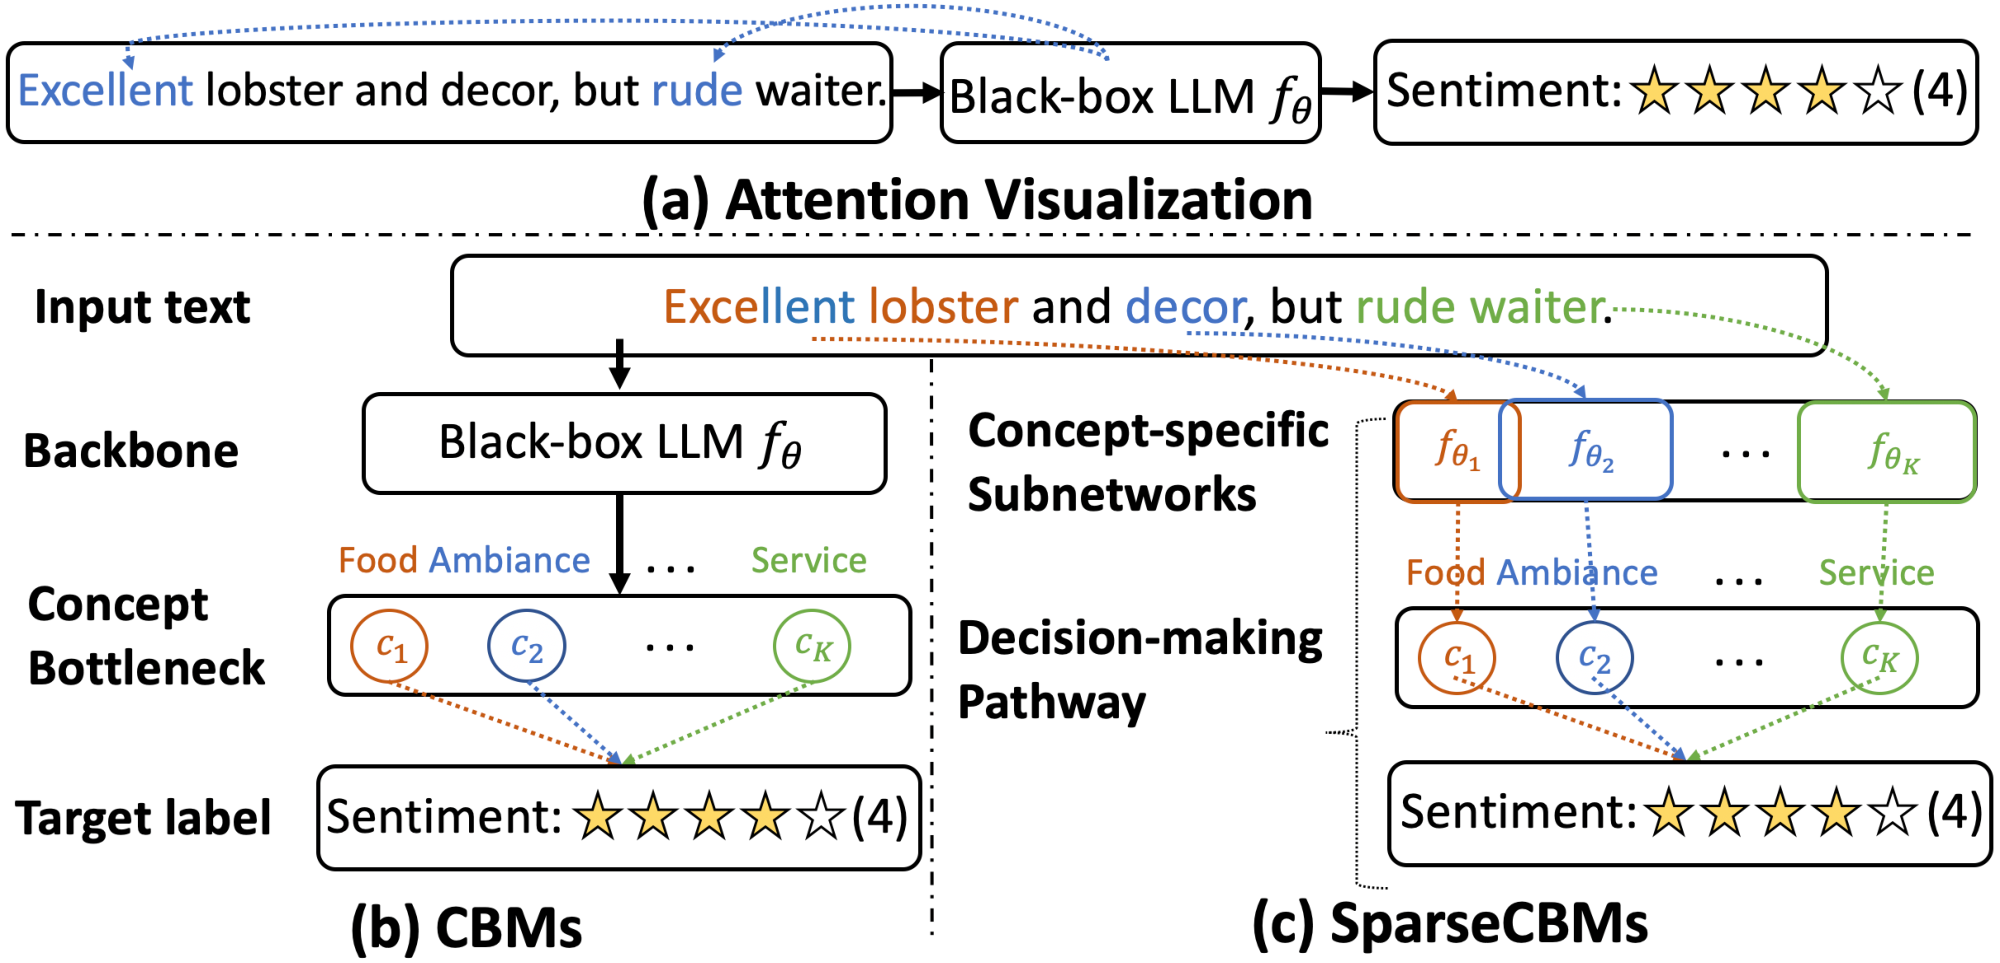
\includegraphics[width=0.8\textwidth]{img/fig1.pdf}}
	%\subcaptionbox{\includegraphics[width=0.48\textwidth]{img/nwaykshot.pdf}}
% %removedVspace
\caption{The illustration includes:
(a) \textit{Attention visualization} provides a localized, attention-driven explanation. While insightful, this might be less decipherable or intuitive for users outside the realm of computer science.
(b) \textit{CBMs} deliver a broader, concept-level understanding, resonating naturally with human cognition. However, they sometimes miss out on the nuanced, granular insights of the LLM's workings.
(c) \textit{SparseCBMs} outline a holistic decision pathway for each input, seamlessly progressing from tokens, via pertinent subnetworks and concepts, to the final task label. This approach marries the strengths of both local and global explanations, addressing their respective shortcomings.}
% %removedVspace
\label{fig:teaser}
	\end{figure}

The spectrum of interpretability solutions for language models can be broadly bifurcated into two categories.
\ding{182}~Initial approaches predominantly leverage \textit{local explanations}, employing techniques such as visualization of attention weights~\cite{galassi2020attention}, probing of feature representations~\cite{mishra2017local,lundberg2017unified}, and utilization of counterfactuals~\cite{wu2021polyjuice,ross2021explaining}, among others.
These methods focus on providing explanations at granular levels, such as individual tokens, instances, neurons, or subnetworks, as exemplified in Figure~\ref{fig:teaser}~(a). While these low-level explanations offer a degree of reliability, they often sacrifice \textbf{readability} and \textbf{intuitiveness}~\citep{losch2019interpretability}, thereby constraining their practical applicability. \ding{183}~More recently, researchers have tended to \textit{global explanations}, such as concept-based analyses that inherently resonate with human cognition~\citep{wang2023intepreting,abraham2022cebab}. For instance, one recent work~\citep{tan2023cbm} incorporates Concept Bottleneck Models (CBMs)~\citep{koh2020concept} into pretrained language models, leading to an impressive ``interpretability-utility'' Pareto front. Figure~\ref{fig:teaser} (b) exemplifies this for sentiment analysis tasks, where human-intelligible concepts like ``Food'', ``Ambiance'', and ``Service'' correspond to neurons in the concept bottleneck layer. The final decision layer is designed as a linear function of these concepts, rendering the decision rules easily understandable. However, these methods excessively focus on global explanations. The \textbf{underlying reasoning} between raw input and concepts remains unclear.
% , especially for LLMs hosting billions of parameters.

% . Moreover, interpretability remains underexplored for the realm of large language models, specifically those encompassing billions of parameters, presenting a clear gap in our understanding of these powerful models.

To address these limitations, our work champions a \textit{holistic} interpretation of LLM predictions. We unveil \textit{SparseCBM}, an evolved CBM variant that melds the complementary ``strengths'' of local and global explanations, thereby addressing the individual ``weaknesses'' of each. This confluence is born from rigorous sparsity-guided refinement designed specifically for LLMs, as depicted in Figure~\ref{fig:teaser} (c). Concretely, SparseCBM iteratively prunes the LLM backbone guided by a joint objective of optimizing for both concept and task labels until the desired sparsity level is accomplished. This exercise distills the LLM into distinct yet interconnected subnetworks, each corresponding to a predefined concept. As such, SparseCBM provides a comprehensive and intelligible decision-making pathway for each input text, tracing from tokens through subnetworks and concepts, ultimately leading to the final task label.

Another unique feature is that, SparseCBMs allow \textbf{interpretable inference-time intervention}~\citep{koh2020concept,li2023inference}. The inherent sparsity-driven structure of SparseCBM allows it to adjust its internal parameters dynamically, based on the context of the input. In practical terms, this means that, during inference, SparseCBM can identify potential areas of ambiguity or misconception, and proactively modify its internal decision-making routes without a full-scale retraining. This ``on-the-fly'' adaptability not only enhances prediction accuracy but also offers users a window into how the model adjusts its reasoning in real time. By making these modifications both accessible and understandable, SparseCBM bridges the common chasm between interpretability and agility for LLMs. This real-time decision pathway modification,
% grounded in comprehensible concepts,
stands as a beacon for fostering trust and facilitating more nuanced human-model interactions. In summary, SparseCBM carries the following advantages:
\begin{itemize}
    \item \underline{\textit{Empirical Validation}}: Our experiments reveal that SparseCBM enables interpretability at the token, subnetwork, and concept levels, creating a synergy that surpasses the mere aggregation of these elements.
    \item \underline{\textit{Superior Performance}}: SparseCBM demonstrates state-of-the-art performance on conventional benchmarks, both in terms of concept and task label predictions.
    \item \underline{\textit{Metacognitive Inference-Time Intervention}}: Compared to vanilla CBMs, SparseCBM exhibits a unique capability for efficient and interpretable inference-time intervention. By subtly modulating internal sparsity, SparseCBM learns to sidestep known pitfalls. This property bolsters user trust in SparseCBMs and, by extension, LLMs.

    % \item Experimentally, we exihbit that SparseCBM facilitates interpretation at the input, subnetwork, and concept levels, leading to a synergy that transcends the mere aggregation of its individual parts;
    % \item We further demonstrate that SparseCBM obtains state-of-the-art results on standard benchmarks in terms of both concept and task label prediction;
    % \item A unique feature of SparseCBM, compared to conventional CBMs, lies in its capacity for efficient and interpretable inference-time intervention~\citep{koh2020concept,li2023inference}. Through the modulation of internal sparsity, SparseCBM can learn to circumvent previously encountered errors without necessitating retraining of the LLM backbone. This feature serves to bolster the trust of envisioning users in SparseCBM and, by extension, LLMs.
\end{itemize}









\section{Related Work}
\subsection{Interpreting Language Models}
Research on the interpretability of language models has been robust, with previous work focusing on visualization of hidden states and attention weights in transformer-based models~\cite{vig2019multiscale,galassi2020attention}. These techniques, while valuable, often provided granular insights that were not easily interpretable at a high level. Feature importance methods like LIME~\cite{ribeiro2016should} and SHAP~\cite{lundberg2017unified} provided valuable insights into how each input feature contributes to the prediction, but still fail to offer a global understanding of the model behavior, and often lack intuitiveness and readability.

The advent of concept-based interpretability has marked a significant development, offering more global, high-level explanations~\cite{koh2020concept,abraham2022cebab,wang2023intepreting}. Concept Bottleneck Models (CBMs)~\citep{koh2020concept,oikarinenlabel} which incorporate a concept layer into the model, have gained traction recently~\cite{tan2023cbm}. CBMs are trained with task labels and concept labels either \textit{independently}, \textit{sequentially}, or \textit{jointly}. This design enables inference-time debugging by calibrating the activations of concepts. Yet, current CBMs are deficient in their ability to offer granular interpretations, and inference-time interventions remain incapable of altering the language model backbone, leading to recurrent errors. On the other hand, the interpretability of LLMs remains a less explored area. Although some progress has been made, such as guiding LLMs to generate explanations for their predictions using finely tuned prompts~\citep{li2022explanations}, the reliability of these explanations remains questionable. In summary, a reliable method facilitating holistic insights into model behavior is still wanting. In response, our work advances this field by introducing SparseCBM, a holistic interpretation framework for LLMs that tackles both local and global interpretations, thus enhancing the usability and trustworthiness of LLMs.


\subsection{Sparsity Mining for Language Models}
Sparsity-driven techniques, often associated with model pruning, form an energetic subset of research primarily in the pursuit of model compression. At their core, these methods focus on the elimination of less influential neurons while retaining the more critical ones, thereby sustaining optimal model performance~\citep{lecun1990optimal,han2015deep,magnitude,hessian,liu2017learning,he2017channel,zhou2016less}. Contemporary research has shed light on the heightened robustness of pruned models against adversarial conditions, such as overfitting and distribution shifts.
Typical pruning methods for language models encompass structured pruning~\citep{michel2019sixteen}, fine-grained structured pruning~\citep{lagunas2021block}, and unstructured pruning~\citep{gale2019state}. In brief, unstructured pruning removes individual weights in a network, leading to a sparse matrix, structured pruning eliminates entire structures like neurons or layers for a dense model, while fine-grained structured pruning prunes smaller structures like channels or weight vectors, offering a balance between the previous two. We direct the readers to the benchmark~\cite{liu2023sparsity} for a comprehensive overview. In our case, we focus on unstructured pruning for its effectiveness and better interpretability.

Recently, studies have underscored the interpretability afforded by sparse networks~\citep{subramanian2018spine}. For instance, \citet{meister2021sparse} delve into the interpretability of sparse attention mechanisms in language models, \citet{liu2022improve} incorporate sparse contrastive learning in an ancillary sparse coding layer to facilitate word-level interpretability, and \citet{oikarinenlabel} demonstrate that a sparsity constraint on the final linear predictor enhances concept-level interpretation of CBMs. Despite their effectiveness, these frameworks restrict sparsity to a handful of layers, leading to unidimensional interpretability that falls short of the desired comprehensiveness. In contrast, our proposed framework, SparseCBM, imposes sparsity across the entire LLM backbone, enabling holistic interpretation at the token, subnetwork, and concept levels.

\section{Methodology}
\subsection{Preliminary: Concept Bottleneck Models for Language Models
}
\subsubsection{Problem Setup.}\label{sec:setup}
In this study, we aim to interpret the predictions of fine-tuned Large Language Models (LLMs) in text classification tasks. Given a dataset $\mathcal{D} = \{(\bm{x}^{(i)}, y^{(i)}, \bm{c}^{(i)})_{i=1}^N\}$, we consider an LLM $f_{\bm{\theta}}$ that encodes an input text $\bm{x} \in \mathbb{R}^D$ into a latent representation $\bm{z} \in \mathbb{R}^E$, and a linear classifier $g_{\bm{\phi}}$ that maps $\bm{z}$ into the task label $y$.

\subsubsection{Incorporate Concept Bottlenecks for Large Language Models.} Our architecture mainly follows \citet{tan2023cbm}. Instead of modifying LLM encoders, which could significantly affect the quality of the learned text representation, we introduce a linear layer with sigmoid activation $p_{\bm{\psi}}$. This layer projects the learned latent representation $\bm{z} \in \mathbb{R}^E$ into the concept space $\bm{c} \in \mathbb{R}^K$, resulting in a pathway represented as $\bm{x} \rightarrow \bm{z} \rightarrow \bm{c} \rightarrow y$. Here, we allow multi-class concepts for more flexible interpretation. For convenience, we represent CBM-incorporated LLMs as LLM-CBMs (e.g., BERT-CBM). LLM-CBMs are trained with two objectives: (1) align concept prediction $\hat{\bm{c}}=p_{\bm\psi}(f_{\bm\theta}(\bm{x}))$ to $\bm{x}$’s ground-truth concept labels $\bm{c}$, and (2) align label prediction $\hat{y}=g_{\bm\phi}(p_{\bm\psi}(f_{\bm\theta}(\bm{x})))$ to ground-truth task labels $y$. We mainly experiment with our framework optimized through the \textit{joint training} strategy for its significantly better performance, as also demonstrated in~\citet{tan2023cbm}.
Jointly training LLM with the concept and task labels entails learning the concept encoder and label predictor via a weighted sum, $\mathcal{L}_{joint}$, of the two objectives:
\begin{equation} \label{eq:joint}
\begin{aligned}
    \bm{\theta}^{\ast}, \bm{\psi}^{\ast}, \bm{\phi}^{\ast} &= \argmin_{\bm{\theta}, \bm{\psi}, \bm{\phi}} \mathcal{L}_{joint}(\bm{x}, \bm{c}, y) \\ &= \argmin_{\bm{\theta}, \bm{\psi}, \bm{\phi}} [\mathcal{L}_{CE} (g_{\bm{\phi}}(p_{\bm{\psi}}(f_{\bm{\theta}}(\bm{x}),y) \\ &\quad+ \gamma \mathcal{L}_{CE} (p_{\bm{\psi}}(f_{\bm{\theta}}(\bm{x})),\bm{c})].
\end{aligned}
\end{equation}
It's worth noting that the LLM-CBMs trained jointly are sensitive to the loss weight $\gamma$. We set the default value for $\gamma$ as $5.0$ for its better performance~\citep{tan2023cbm}. Despite the promising progress having been made, present LLM-CBMs typically train all concepts concurrently, leading to intertwined parameters for concept prediction, making the process less transparent and hampering targeted intervention.

\subsection{\textit{SparseCBMs}}
To address the aforementioned issue, the goal of this paper is to provide a holistic and intelligible decision-making pathway for each input text, tracing from tokens through subnetworks and concepts, ultimately leading to the final task label.
To this end, we introduce \textit{SparseCBM}, a pioneering framework capable of unraveling the intricate LLM architectures into a number of concept-specific subnetworks. Our approach not only outperforms conventional CBMs in concept and task label prediction performance but also proffers enhanced interpretation concerning neuron activations, for instance, illuminating which weights inside the LLM backbone play pivotal roles in learning specific concepts.

Our framework starts with decomposing the joint optimization defined in Eq.~\eqref{eq:joint} according to each concept $c_k$, which is formulated as follows:
\begin{equation}\label{eq:decompose}
\begin{aligned}
    \bm{\theta}^{\ast}, \bm{\psi}^{\ast}, \bm{\phi}^{\ast} &= \{(\bm\theta^{\ast}_k)_{k=1}^{K}\}, \{(\bm\psi^{\ast}_k)_{k=1}^{K}\}, \{(\bm\phi^{\ast}_k)_{k=1}^{K}\} \\ &= \argmin_{\bm\theta, \bm\psi, \bm\phi} \sum_{k=1}^K \mathcal{L}_{joint}(\bm{x}, c_k, y). \\
    &= \argmin_{\bm\theta, \bm\psi, \bm\phi} \sum_{k=1}^K [\mathcal{L}_{CE} (g_{\bm{\phi}_k}(p_{\bm{\psi}_k}(f_{\bm{\theta}}(x),y) \\ &\quad+ \gamma \mathcal{L}_{CE} (p_{\bm{\psi}_k}(f_{\bm{\theta}}(\bm{x})),c_k)],
\end{aligned}
\end{equation}
where $\bm{\phi}_k, \bm{\psi}_k$ are the weights of the $k$th parameter of the projector and classifier, and $\bm{\theta}_k$ is the subnetwork specific for the concept $c_k$, which is explained later. Since both of them are comprised of a single linear layer (with or without the activation function), the involved parameters for $c_k$ can be directly indexed from these models and are self-interpretable~\cite{koh2020concept,tan2023cbm}.

The remaining task is to excavate concept-specific subnetworks for each concept from the vast architecture of Large Language Models (LLMs). The guiding intuition behind this strategy is to perceive the prediction of concept labels as individual classification tasks, ones that should not strain the entirety of pretrained LLMs given their colossal reserves of knowledge encapsulated in multi-million to multi-billion parameters. We propose an unstructured pruning of the LLM backbone for each concept classification task, such that distinct pruned subnetworks are accountable for different concepts while preserving prediction performance.
% Our experiments show that, a pruned SparseCBM model with $\frac{1}{K}$ parameters can even ourperform its dense counterpart.

\subsubsection{Holistic and Intelligible Decision-making Pathways.}
% This work principally aims to mine concept-specific subnetworks for each concept from the vast architecture of Large Language Models (LLMs). The guiding intuition behind this approach is the interpretation of each concept label prediction as an individual classification task, which should be an endeavor that should pose minimal challenge to pretrained LLMs, given their multimillion to multibillion parameter range.

We leverage unstructured pruning strategies to carve out concept-specific subnetworks within the LLM backbones. The noteworthy edge of such unstructured pruning strategies lies in their ability to engender weight masks in accordance with the weight importance. Such masks naturally can offer an immediate and clear interpretation. Concretely, we introduce a 0/1 weight mask $M_k$ for each corresponding subnetwork. Consequently, the weights of each subnetwork can be represented as $\bm{\theta}_{\bm{M}_k} = \bm{M}_k \odot \bm{\theta}^\ast$, representing the Hadamard (element-wise) product between the LLM weights $\bm{\theta}^{\ast} \in \mathbb{R}^L$ and the weight mask $\bm{M}_k \in \{0,1\}^L$ for the concept $c_k$.

With well-optimized $\{(\bm{M})_{k=1}^K\}$, during inference, the decision-making pathway can be represented as:
\begin{equation}\label{eq:path}
    \hat{y} = \sum_{k=1}^{K} \bm{\phi}_k^\ast \cdot \sigma(\bm{\psi}_k^\ast \cdot f_{\bm{\theta}_{\bm{M}_k}} (\bm{x})) = \sum_{k=1}^{K} \bm{\phi}_k^\ast \cdot \sigma(\bm{\psi}_k^\ast \cdot f_{\bm{M}_k^ \odot \bm{\theta}^\ast} (\bm{x})),
\end{equation}
where $\sigma(\cdot)$ is the sigmoid activation function of the projector. This decision-making pathway defined in Eq.~\eqref{eq:path} factorizes the parameters of the SparseCBM, and can be optimized through one backward pass of the discomposed joint loss defined in Eq.~\eqref{eq:decompose} with $\bm{\theta}_k^\ast = \bm{\theta}_{\bm{M}_k}$. Importantly, we posit that such decision-making pathways can deliver holistic explanations for the model's predictions. For instance, by scrutinizing the weights in the classifier $g_{\bm{\phi}}$ and the concept activation post the $\sigma$ function, we can get a concept-level explanation regarding the importance of different concepts. Also, visualizing each subnetwork mask $\bm{M}_k$ will furnish a subnetwork-level comprehension of neuron behavior and its importance in acquiring a specific concept and forming predictions. Additionally, the study of the gradient of input tokens in masked concept-specific subnetworks can provide more accurate token-concept mapping. Notably, our experiments demonstrate that SparseCBMs, in addition to providing multi-dimensional interpretations, can match or even surpass their dense counterparts in performance on both concept and task label prediction.
Another unique feature of SparseCBMs lies in that, the weight masks $\{(\bm{M}_k)_{k=1}^K\}$ engendered by unstructured pruning facilitates the process of efficient and interpretable \textit{Sparsity-based Inference-time Intervention}, which is expounded later.


\subsubsection{Concept-Induced Sparsity Mining.}
Next, we elaborate on how to compute those sparsity masks, given an optimized LLM backbone. A second-order unstructured pruning~\cite{hassibi1992second,kurtic2022optimal} for LLMs has been incorporated. Initially, the joint loss $\mathcal{L}$ (we omit the subscript $joint$ for brevity in subsequent equations) can be expanded at the weights of subnetwork $\bm{\theta}_{\bm{M}_k}$ via Taylor expansion:
% \begin{align}
%     \mathcal{L}(\bm{\theta}_{\bm{M}_k}) &\simeq \mathcal{L}(\bm{\theta}^\ast) + (\bm{\theta}_{\bm{M}_k} - \bm{\theta}^\ast)^{\top} \nabla \mathcal{L}(\bm{\theta}^\ast) \nonumber\\&+ \frac{1}{2}(\bm{\theta}_{\bm{M}_k}-\bm{\theta}^\ast)^\top \bm{H}_{\mathcal{L}} (\bm{\theta^\ast})(\bm{\theta_{\bm{M}_k}})
% \end{align}
\begin{equation}
\begin{aligned}
    \mathcal{L}(\bm{\theta}_{\bm{M}_k}) &\simeq \mathcal{L}(\bm{\theta}^\ast) + (\bm{\theta}_{\bm{M}_k} - \bm{\theta}^\ast)^{\top} \nabla \mathcal{L}(\bm{\theta}^\ast) \\& \quad+ \frac{1}{2}(\bm{\theta}_{\bm{M}_k}-\bm{\theta}^\ast)^\top \bm{H}_{\mathcal{L}} (\bm{\theta}^\ast)(\bm{\theta_{\bm{M}_k}} - \bm{\theta}^\ast),
\end{aligned}
\end{equation}
where $\bm{H}_{\mathcal{L}}(\bm{\theta}^\ast)$ stands for the Hessian matrix of the decomposed joint loss at $\bm{\theta}^\ast$. Since $\bm{\theta}^\ast$ is well-optimized, we assume $\nabla \mathcal{L} (\bm{\theta}^\ast) \approx 0$ as the common practice~\cite{hassibi1992second,kurtic2022optimal}. Then, the change in loss after pruning can be represented as:
\begin{equation}
    \Delta \mathcal{L} (\Delta\bm\theta) = \mathcal{L}(\bm{\theta}_{\bm{M}_k}) - \mathcal{L} (\bm\theta^\ast) \simeq \frac{1}{2}\Delta\bm\theta^\top \bm{H}_\mathcal{L} \Delta \bm{\theta},
\end{equation}
where, $\Delta\bm{\theta} = \bm\theta_{\bm{M}_k}-\bm{\theta}^\ast$ signifies the change in LLM weights, that is, pruned parameters. Given a target sparsity $s\in [0,1)$, we seek the minimum loss change incurred by pruning. In our case, the default sparsity is designed as: $s \geq 1-\frac{1}{K}$, implying each subnetwork contains a maximum of $\frac{1}{K}$ parameters in the dense counterpart. Ideally, we desire separate parameters in the LLM backbone to ensure optimal interpretability. Then, the problem of computing the sparsity masks can be formulated as a constrained optimization task:
\begin{equation}\label{eq:optimization}
    \begin{aligned}
        &\min_{\Delta \bm\theta} \quad \frac{1}{2} \Delta \bm{\theta}^\top \bm{H}_{\mathcal{L}} (\bm{\theta^\ast}) \Delta \bm\theta,
        \\& s.t. \quad \bm{e}_b^{\top} \Delta \bm\theta + \theta_b = 0, \quad \forall b \in \bm{Q},
    \end{aligned}
\end{equation}
where $\bm{e}_b$ denotes the $b$th canonical basis vector of the block of weights $\bm{Q}$ to be pruned.
This optimization can be solved by approximating the
Hessian at $\bm\theta^\ast$ via the dampened empirical Fisher
information matrix~\citep{hassibi1992second,kurtic2022optimal}. Hence, we can derive the optimized concept-specific masks $\{(\bm{M}_k)_{k=1}^K\}$. More details are in Appendix C.


% For convenience, we use BERT models to represent BERT-family models. As described in the previous section, our goal is to extract a dedicated subnetwork from the BERT model for each concept. To achieve this, we first decompose the training with joint loss according to each concept $c_k$ as follows:
% \begin{equation}
%     \theta^{\ast}, \psi^{\ast}, \phi^{\ast} &= \theta^{\ast}, \psi^{\ast}, \phi^{\ast}

%     \argmin_{\theta, \psi_k, \phi_k} \mathcal{L}_{joint}(x, c_k, y).
% \end{equation}



% , firstly, we train the BERT model for a specifc concept $c_k, \forall k \in \{1,2,\ldots,K\}$ through the standard joint training strategy. Note that during this training, inside the projector $p_\psi$ and the classifier $g_\phi$, since both of them are linear layers, only the weights corresponding to $c_k$, i.e., $\psi_k, \phi_k$, are updated.
% % The final loss is the sum of losses from all the concepts.
% Then, through the predefined loss $\mathcal{L}_{joint}$, we can get the well-optimized dense BERT model with weights $\theta^{\ast}$:
% \begin{equation}
%     \theta^{\ast}, \psi^{\ast}_k, \phi^{\ast}_k &= \argmin_{\theta, \psi_k, \phi_k} \mathcal{L}_{joint}(x, c_k, y).
% \end{equation}

\subsubsection{Sparsity-based Inference-time intervention.} SparseCBMs also exhibit the capability to allow inference-time concept intervention (a trait inherited from CBMs), thus enabling more comprehensive and user-friendly interactions.
SparseCBMs allow modulation of the inferred concept activations: $\hat{\bm{a}} = \sigma (p_{\bm\phi}(f_{\bm{\theta}}(\bm{x})))$. There are two straightforward strategies for undertaking such intervention. The first option is the \textit{oracle intervention}~\citep{koh2020concept}, where human experts manually calibrate the concept activations $\hat{\bm{a}}$ and feed them into the classifier.
% In practical scenarios, domain experts interacting with the model might intervene to ``correct'' any potentially erroneous concept activations predicted by the model.
Despite its apparent simplicity, oracle intervention directly operates on concept activations and, therefore, cannot fix the flawed mapping learned by the LLM backbone. As a consequence, the model will replicate the same error when presented with the same input. Meanwhile, another strategy involves further fine-tuning the LLM backbone on the test data. However, this approach is not only inefficient but also has a high risk of leading to significant overfitting on the test data. Those limitations present a barrier to the practical implementation of CBMs in high-stakes or time-sensitive applications.

As a remedy, we further propose a \textit{sparsity-based intervention} that is self-interpretable and congruent with SparseCBMs. It helps LLMs to learn from each erroneously predicted concept during inference time, while preserving overall performance. The core idea is to subtly modify the concept-specific masks for the LLM backbone when a mispredicted concept is detected. Specifically, parameters of the LLM backbone $f_\theta$, projector $p_\psi$, and the classifier $g_\phi$ are frozen, while the concept-specific masks $\{(\bm{M}_k)_{k=1}^K\}$ is kept trainable. During the test phase, if a concept prediction $\hat{c}_k$ for an input text $\bm{x}$ is incorrect, we acquire the gradient ${\mathcal{G}_k}(\bm{x})$ for the corresponding subnetwork $f_{\bm{\theta}_{\bm{M}_k}}$, and modulate the learned mask $\bm{M}_k$ accordingly.

Inspired by~\citet{evci2020rigging,sun2023simple}, we define the saliency scores for LLM parameters by the $l_2$-norm of the product of the gradient of the mask and the parameter weights: $\mathcal{S} = \|\mathcal{G}_k(\bm{x}) \cdot \bm{\theta}^\ast \|$. Subsequently, we perform the following two operations based on the saliency scores: (1)~\textbf{Drop} a proportion of $r$ unpruned weights with the lowest saliency scores: $\argmin_m^{r\cdot |\bm{\theta}|} \mathcal{S}_m$, $\forall m \in |\bm{\theta}_{\bm{M}_k}|$. (2) \textbf{Grow} a proportion of $r$ pruned weights with the highest saliency scores: $\argmax_m^{r\cdot |\bm{\theta}|} \mathcal{S}_m$, $\forall m \in |\bm{\theta} \setminus \bm{\theta}_{\bm{M}_k}|$. Here $m$ refers to the parameter index of the LLM backbone. By dropping and growing an equal number of parameters, the overall sparsity $s$ of the LLM backbone remains unchanged. This mask-level intervention is further optimized through the decomposed joint loss $\mathcal{L}_{joint}$ defined in Eq.~\eqref{eq:decompose}. Note that $r$ is set as a relatively small value (e.g., 0.01) to compel the model to retain the overall performance while learning from the mistake. Our experiments validate that the proposed sparsity-based intervention can effectively enhance inference-time accuracy without necessitating training of the entire LLM backbone. Also, the intervened parameters provide insight into the parameters that contributed to each misprediction.





\section{Experiments}
\subsection{Experimental Setup}
\subsubsection{Datasets.} Our experiments are conducted on two widely-used real-world datasets: \texttt{CEBaB}~\citep{abraham2022cebab} and \texttt{IMDB-C}~\cite{tan2023cbm}. Each of them is a text-classification dataset comprised of human-annotated concept and task labels. Their statistics are presented in Table~\ref{tab:data}.
\subsubsection{LLM backbones.}
In this research, we primarily consider two widely-recognized, open-source lineages of pretrained LLMs: the BERT-family models~\cite{devlin2018bert,liu2019roberta,sanh2019distilbert} and OPT-family models~\cite{zhang2022opt}. Specially, we also include directly prompting GPT4~\cite{openai2023gpt4} as a baseline to let it generate concept and task labels for given texts.
% Used prompts and more details are included in Appendix B.
Even though being proprietary, GPT4 is widely regarded as the most capable LLM currently, so we choose it as the baseline backbone. For better performance, we obtain the representations of the input texts by pooling the embedding of all tokens. Reported scores are the averages of three independent runs. Our work is based on general text classification implementations. The PyTorch Implementation is available at \textit{https://github.com/Zhen-Tan-dmml/SparseCBM.git}.


\begin{table}[t]
% \scalebox{0.69}{
\centering
% \renewcommand{\arraystretch}{1.5}
\setlength{\tabcolsep}{1pt} % Change 6pt to your desired value
\fontsize{9pt}{10pt}\selectfont
\begin{tabular}{@{}c|cccc@{}}
\toprule
\multirow{2}{*}{\textbf{Dataset}} & \multicolumn{4}{c}{\texttt{CEBaB}    (5-way classification)}                                   \\ \cmidrule(l){2-5}
                                  & \multicolumn{2}{c|}{\textbf{Train/Dev/Test}} & \multicolumn{2}{c}{1755 / 1673 / 1685} \\ \midrule
\multirow{5}{*}{\textbf{Concept}} & \textbf{Concept}      & \textbf{Negative}    & \textbf{Positive}  & \textbf{Unknown}  \\ \cmidrule(l){2-5}
                                  & Food                  & 1693 (33\%)        & 2087 (41\%)      & 1333 (26\%)     \\
                                  & Ambiance              & 787 (15\%)         & 994 (20\%)       & 3332 (65\%)     \\
                                  & Service               & 1249 (24\%)        & 1397 (27\%)      & 2467 (49\%)     \\
                                  & Noise                 & 645 (13\%)         & 442 (9\%)        & 4026 (78\%)     \\ \midrule
\multirow{2}{*}{\textbf{Dataset}} & \multicolumn{4}{c}{\texttt{IMDB-C}    (2-way classification)}                                    \\ \cmidrule(l){2-5}
                                  & \multicolumn{2}{c|}{\textbf{Train/Dev/Test}} & \multicolumn{2}{c}{100 / 50 / 50}      \\ \midrule
\multirow{5}{*}{\textbf{Concept}} & \textbf{Concept}      & \textbf{Negative}    & \textbf{Positive}  & \textbf{Unknown}  \\ \cmidrule(l){2-5}
                                  & Acting                & 76 (38\%)            & 66 (33\%)          & 58 (29\%)         \\
                                  & Storyline             & 80 (40\%)            & 77 (38\%)        & 43 (22\%)       \\
                                  & Emotion     & 74 (37\%)            & 73 (36\%)        & 53 (27\%)       \\
                                  & Cinematography        & 118 (59\%)           & 43 (22\%)        & 39 (19\%)       \\ \bottomrule
\end{tabular}
% %removedVspace
\caption{Statistics of experimented datasets and concepts.}\label{tab:data}
\end{table}

\begin{table}[t]
% %removedVspace
\centering
% %removedVspace
\setlength{\tabcolsep}{1pt} % Change 6pt to your desired value
\fontsize{9pt}{9.5pt}\selectfont
\begin{tabular}{cccccc}
\toprule
\multirow{2}{*}{\textbf{Backbone}}   & \multirow{2}{*}{\textbf{Acc. / F1}} & \multicolumn{2}{c}{\texttt{CEBaB}}                                & \multicolumn{2}{c}{\texttt{IMDB-C}}                                 \\ \cline{3-6}
                                     &                                     & \textbf{Concept}                & \textbf{Task}                   & \textbf{Concept}                & \textbf{Task}                   \\ \midrule
\textbf{GPT4}                        & Prompt                           & \multicolumn{1}{l}{75.9/71.5} & \multicolumn{1}{l}{51.3/45.9} & \multicolumn{1}{l}{64.5/61.5} & \multicolumn{1}{l}{71.4/68.7} \\ \midrule
\multirow{3}{*}{\textbf{DistilBERT}} & Standard                            & -                               & 70.3/80.4                     & -                               &     77.1/73.8                           \\
                                     & CBM                                 & 81.1/83.5                     &  63.9/76.5                     &        67.5/63.8                         & 76.5/69.8                                \\
                                     & SparseCBM                           & \textbf{82.0/84.0}            & \textbf{64.7/77.1}            &     \textbf{68.4/64.3}                            &    \textbf{76.9/71.4}                             \\ \midrule
\multirow{3}{*}{\textbf{BERT}}       & Standard                            & -                               & 67.9/79.8                     & -                               &  78.3/72.1                               \\
                                     & CBM                                 & 83.2/85.3                     & 66.9/78.1                     &   68.2/62.8                              &    77.3/70.4                             \\
                                     & SparseCBM                           & \textbf{83.5/85.6}            & \textbf{66.9/79.1}            &    \textbf{69.8/65.2}                             &    76.5/\textbf{71.6}                             \\ \midrule
\multirow{3}{*}{\textbf{RoBERTa}}    & Standard                            & -                               & 71.8/81.3                     & -                               &   82.2/77.3                              \\
                                     & CBM                                 & 82.6/84.9                     & 70.1/81.3                     &       69.9/68.9                          &     81.4/79.3                            \\
                                     & SparseCBM                           & \textbf{82.8/85.5}            & \textbf{70.3/81.4}            &    \textbf{70.2/69.7}                             &    \textbf{81.5/79.9}                             \\ \midrule
\multirow{3}{*}{\textbf{OPT-125M}}   & Standard                            & -                               & 70.8/81.4                     & -                               &    84.3/80.0                             \\
                                     & CBM                                 & 85.4/87.3                     & 68.9/79.7                     &   68.7/66.5                              &      81.8/78.2                           \\
                                     & SparseCBM                           & \textbf{86.2/88.0}            & \textbf{68.9/79.8}            &    \textbf{70.0/67.4}                             &     \textbf{82.6/79.9}                            \\ \midrule
\multirow{3}{*}{\textbf{OPT-350M}}   & Standard                            & -                               & 71.6/82.6                     & -                               &        86.4/83.5                         \\
                                     & CBM                                 & 87.8/89.4                     & 69.9/80.7                     &   72.6/70.5                              &      84.5/82.4                           \\
                                     & SparseCBM                           & {87.3/88.7}            & {68.2/79.8}            &     \textbf{73.3/71.1}                            &     \textbf{85.0/82.5}                            \\ \midrule
\multirow{3}{*}{\textbf{OPT-1.3B}}   & Standard                            & -                               & 74.7/83.9                     & -                               &       88.4/83.7                          \\
                                     & CBM                                 & 90.0/91.5                     & 73.6/82.1                     &   76.8/74.6                              &      85.7/83.3                           \\
                                     & SparseCBM                           & 89.9/\textbf{91.6}            & \textbf{73.8/82.6}            &   76.4/\textbf{74.7}                              &      \textbf{86.6/83.9}                           \\ \bottomrule
\end{tabular}
% %removedVspace
\caption{Comparisons of task accuracy and interpretability using \texttt{CEBaB} and \texttt{IMDB-C} datasets with BERT-family and OPT-family models as the backbones. Metrics for both task and concept labels are \textit{Accuracy}/\textit{Macro F1} in $\%$. A score in \textbf{bold} indicate that the SparseCBM under the current setting outperforms its dense CBM counterpart.}\label{tab:compare}
\end{table}

\subsection{Interpretability}
\subsubsection{Utility v.s. Interpretability.}
Table~\ref{tab:compare} presents the performance of the concept and task label prediction:
\begin{itemize}
    \item \textbf{Multidimensional Interpretability:} SparseCBMs stand out by offering multidimensional interpretability without compromising task prediction performance. In comparison with standard LLMs (which are fine-tuned exclusively with task labels), SparseCBMs grant concept-level interpretability with only a slight dip in task prediction accuracy. Impressively, SparseCBMs can match or even outperform their dense CBM counterparts while providing multifaceted explanations that extend beyond mere concepts. This underlines the potency of SparseCBMs in striking a balance between interpretability and utility.
    \item \textbf{Scalability with Larger LLM Backbones:} The utilization of larger LLMs within SparseCBMs leads to superior interpretability-utility Pareto fronts. This observation validates our guiding hypothesis that predicting concept labels should not strain the entirety of pretrained LLMs as they are individual classification tasks. Larger LLMs, being repositories of more knowledge through increased parameters, facilitate easier pruning.
    % We discuss the potential of larger LLMs for pruning in sensitivity analyses.
    \item \textbf{Limitations of Direct Prompting:} When directly prompting LLMs, such as GPT4 (without fine-tuning on the target datasets), to predict concept and task labels, the resulting performance is noticeably inferior. This highlights the necessity of learning concepts and task labels in target domains. Additionally, since LLMs' task predictions are autoregressively generated and do not rely entirely on the generated concepts, doubts arise regarding the reliability of concept-level explanations.
    % This further validates the necessity of this research.
\end{itemize}



\begin{figure}[b]
% %removedVspace
  \centering
  \scalebox{1}{
                  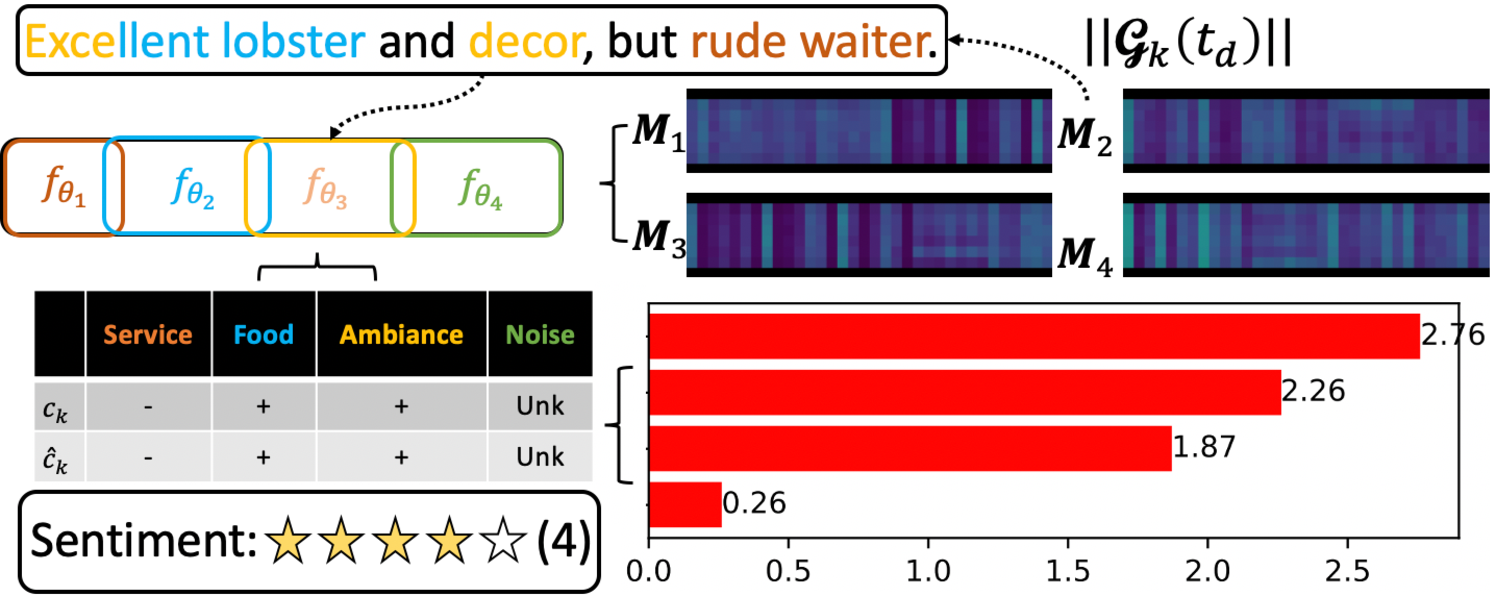
\includegraphics[width=\linewidth]{img/fig2.pdf}}
  % %removedVspace
  \caption{{The illustration of a decision pathway of a toy example from the SparseCBM framework with BERT as the backbone. The binary weight masks for each concept is represented as a heatmap.}}\label{fig:example}
  % %removedVspace
\end{figure}

\subsubsection{Explainable Prediction Pathways.}
The centerpiece of this paper revolves around providing a transparent and interpretive decision-making pathway for each input text vector $\bm{x} = [t_1,t_2,\cdots, t_d,\cdots,t_D]$, where $t_d, \forall d \in D$ denotes the tokens in the input text. SparseCBMs, at inference time, unravel the following layers of understanding across the decision-making trajectory:



\begin{enumerate}
\item \textbf{Subnetwork-Level Explanation:} Identification of specific neurons within the LLM backbones responsible for corresponding concepts. This insight is achieved by visualizing individual binary subnetwork masks
$\bm{M}_k$.
\item \textbf{Token-Level Explanation:} Detection of the tokens instrumental in shaping a particular concept. This analysis is carried out by evaluating the gradient of each subnetwork mask with respect to individual tokens $\|\mathcal{G}_k(t_d)\|$.
\item \textbf{Concept-Level Explanation:} Understanding the predicted concept labels $\hat{c}_k$ and their contribution to the final prediction. This is captured by computing the dot product between each predicted concept activation and the corresponding weight of the linear predictor: $\bm{\phi}_k\cdot\hat{\bm{a}}_k$.
\end{enumerate}
% (1) Subnetwork-level explanation of which neurons in the LLM backbones are responsible for learning the corresponding concepts. This is achieved by visualizing each binary subnetwork mask $\bm{M}_k$ (2) Token-level explanantion on which tokens are responsible for the specific concept. This is achieved by measuring the gradient of each subnetwork mask towards each token $\|\mathcal{G}_k(t_d)\|$. (3) Concept-level explanantion on predicetd concept labels $\hat{c}_k$ and how concepts contribute to the final prediction. This is achieved by measuring the dot product of each predicted concept activation and the corresponding weight of the linear predictor: $\bm{\phi}_k\cdot\hat{\bm{a}}_k$.
A schematic representation of the decision-making process for a representative example is provided in Figure~\ref{fig:example}, with ``Neg Concept'' denoting negative concept values. Additional real-world examples are delineated in Appendix~D. Several interesting findings can be drawn from those results:
\begin{itemize}
\item \textbf{Neural Responsibility Across Concepts:} Various concepts necessitate differing proportions of neurons in the LLM backbone for learning. This resonates with our ambition to demystify the ``black-box'' LLM backbones by partitioning them into distinct subnetworks, each accountable for an individual concept. Intriguingly, overlaps exist among subnetworks, reflecting that strict disentanglement constraints were not imposed on the backbone parameters. This opens avenues for future research into entirely concept-wise disentangled LLM backbones.
\item \textbf{Holistic Decision Pathway:} The SparseCBM framework successfully crafts a comprehensive decision-making path that navigates from tokens, through subnetworks and concepts, culminating in the final task label. This rich interpretability paves the way for unique insights into practical applications. For instance, although concepts like ``Food'' and ``Ambiance'' may carry identical positive values, the ``Food'' concept may wield greater influence on the final task label. Additionally, careful examination of parameter masks can shed light on the root causes behind mispredicted concepts, enabling effective and interpretable interventions. We explore this topic further in the subsequent section.
\end{itemize}


\subsection{Inference-time Intervention}
\begin{figure}[b]
% %removedVspace
		\centering
\captionsetup[sub]{skip=-0.5pt}
\subcaptionbox{Concept Prediction}
{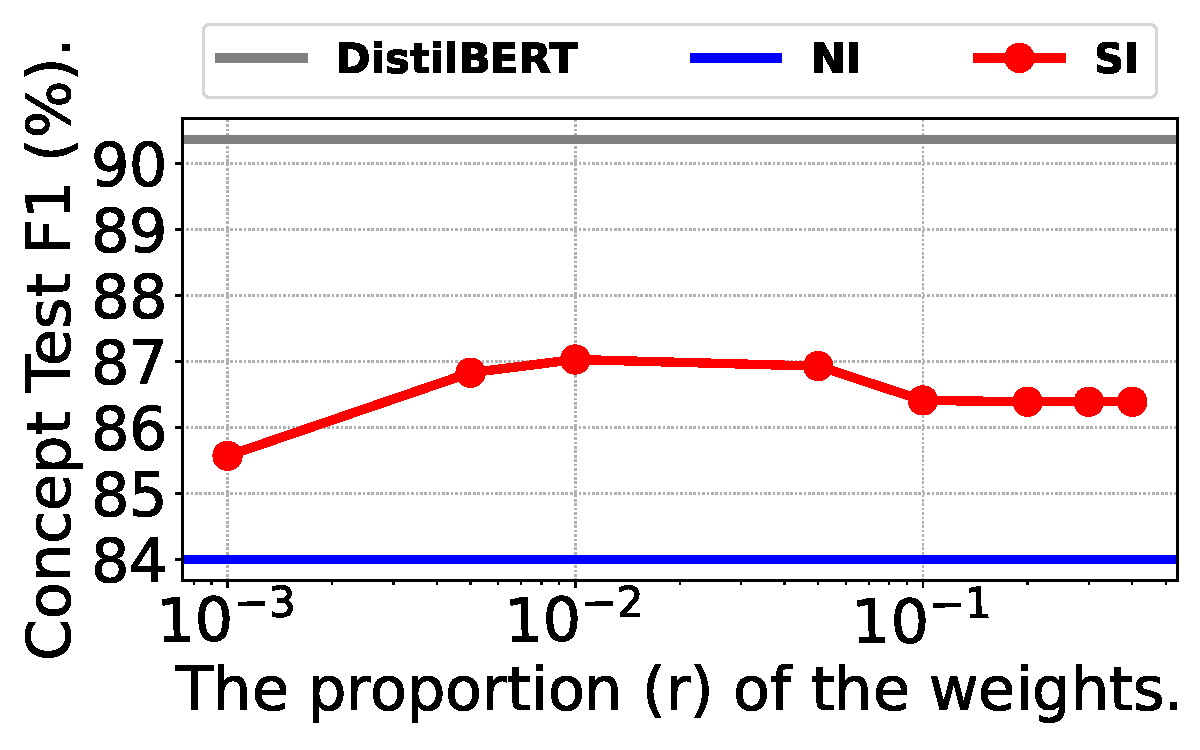
\includegraphics[width=0.225\textwidth]{img/intervene-cebab-concept.pdf}}
\subcaptionbox{{Task Prediction}}
{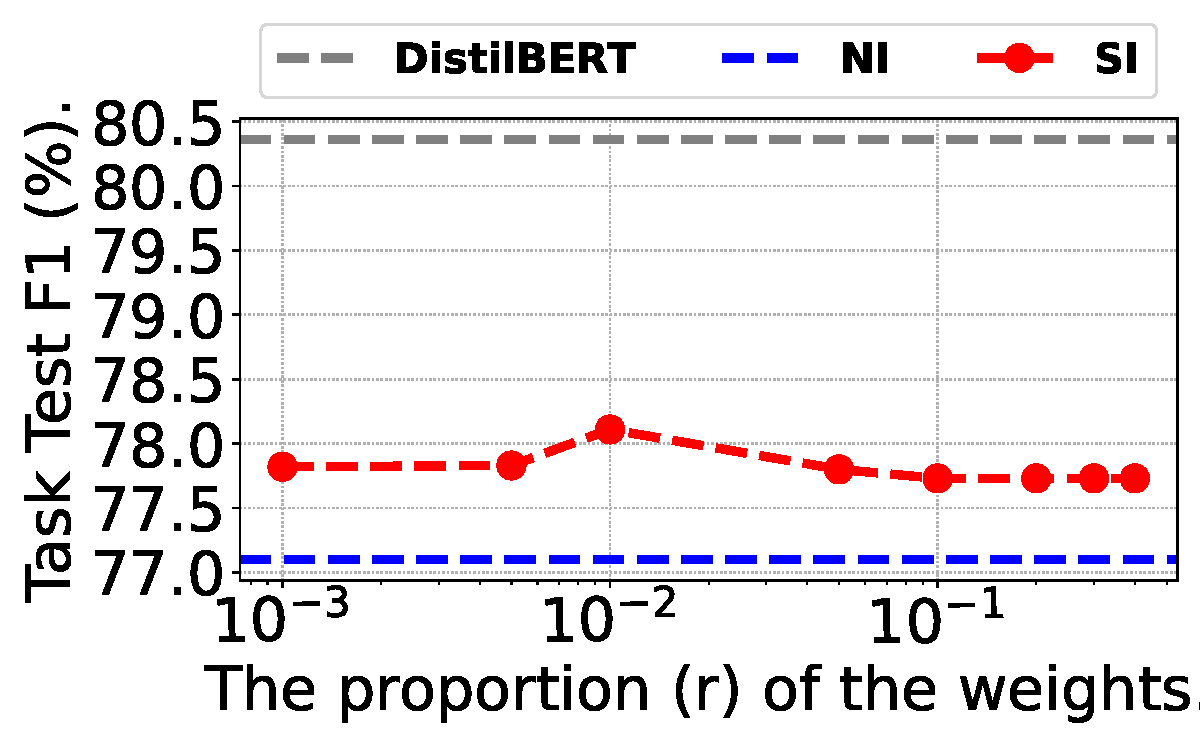
\includegraphics[width=0.225\textwidth]{img/intervene-cebab-task.pdf}}
% %removedVspace
		\caption{The results of Test-time Intervention. ``NI'' denotes ``no intervention'', ``SI'' denotes ``Sparsity-based Intervention''. (a) and (b) represent the results for concept and task label prediction respectively. The x-axis indicates the proportion ($r$) of the weights to perform the intervention.}
		\label{fig:intervene}
% %removedVspace
	\end{figure}
SparseCBMs distinguish themselves by enabling sparsity-based inference-time intervention, compared to vannila CBMs. This innovative feature creates a pathway for more refined, user-centric interactions by subtly adjusting the masks without the need for direct retraining of the LLM backbone. The significance of this intervention approach lies in its application to real-world scenarios where users often find it easier to articulate broad concepts (e.g., food quality) rather than precise sentiment scores or categorical labels.

\subsubsection{Experimental Evaluation.}
To methodically evaluate this intervention strategy, extensive experiments were conducted on the \texttt{CEBaB} dataset, employing DistilBERT as the representative LLM backbone. The insights gleaned from these experiments apply consistently to other LLMs as well. Figure~\ref{fig:intervene} provides a detailed comparison between concept and task label predictions using SparseCBMs against a baseline, where a vanilla DistilBERT is independently trained to classify concept or task labels. These baseline scores serve as a theoretical upper bound for prediction accuracy, providing a reliable and illustrative benchmark.
This analytical exploration not only validates the proposed sparsity-based intervention's efficacy in enhancing inference-time accuracy for both concept and task predictions but also reveals its elegance in execution. With minimal alterations to the underlying model structure, remarkable improvements are achieved. Even for a relatively small model, DistilBERT, the optimal adjustment proportion is found to be a mere $1\%$, translating to modifications in only $2\%$ of the backbone parameters.

\begin{figure}[t]
% %removedVspace
  \centering
  \scalebox{0.95}{
  % \centering
  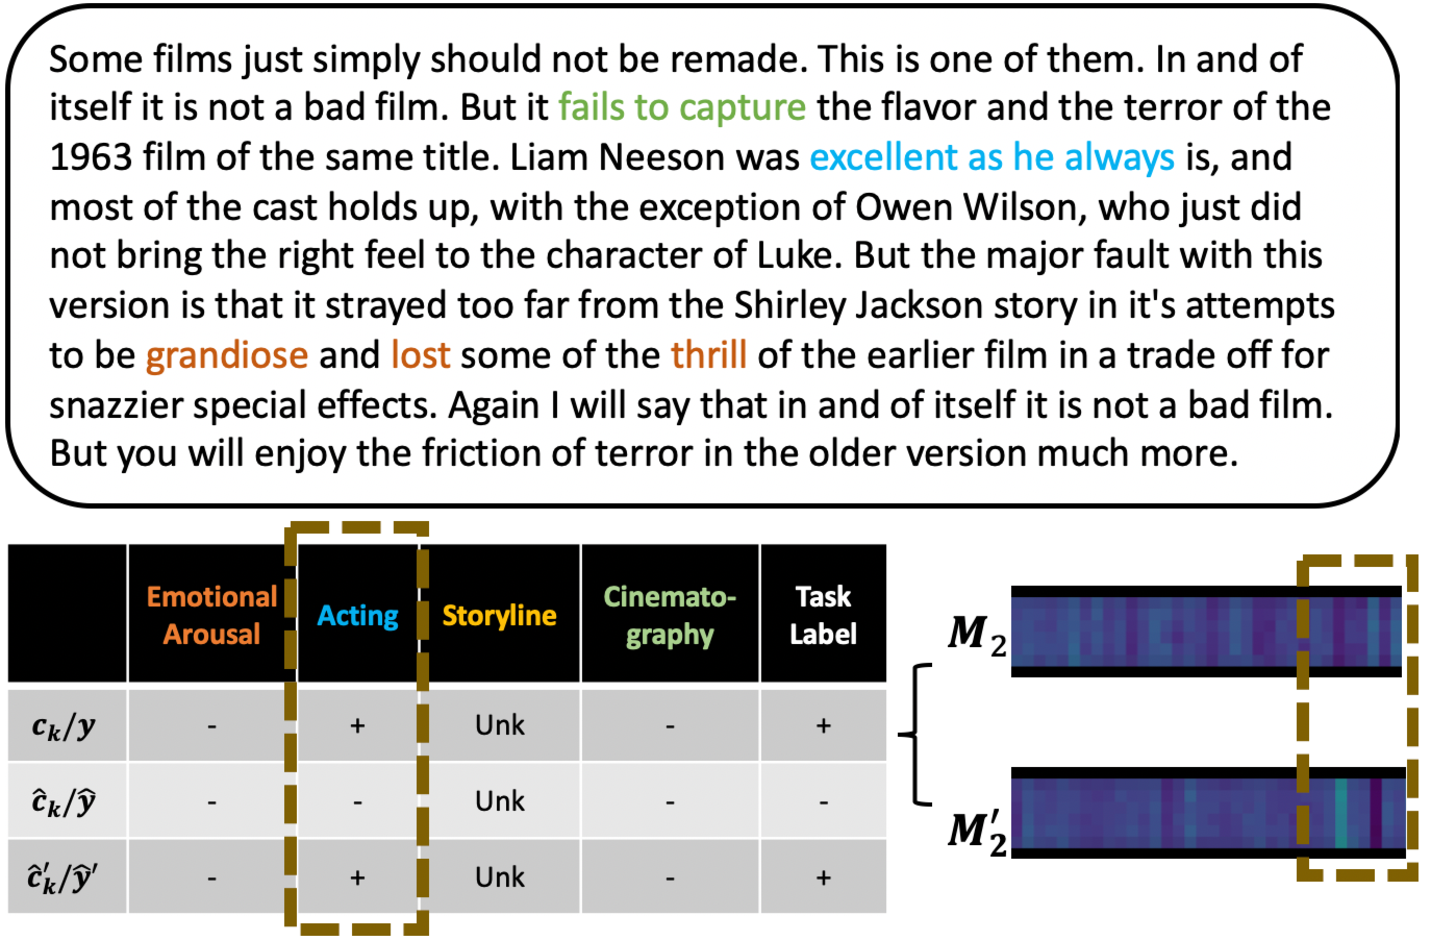
\includegraphics[width=\linewidth]{img/inter.pdf}}
  \caption{Illustration of the explainable prediction for a real-world example from the \texttt{IMDB-C} dataset using OPT-350m as the backbone. The brown boxes with dash lines indicate the test-time intervention on corresponding concepts by modulating the corresponding mask. $\bm{M}_2$ and $\bm{M}_2^\prime$ denote the parameter masks for the second concept, ``Acting'', before and after the intervention, respectively. We visualize $\bm{M}_2^\prime$ after seeing all test samples.}
  \label{fig:inter}
  % %removedVspace
\end{figure}

\subsubsection{Robustness and Adaptability.}
These results shed light on the broader applicability and resilience of sparsity-based intervention across various contexts and domains. The capacity to implement such nuanced adjustments without the resource-intensive process of retraining the entire model marks a substantial advancement toward more agile, responsive machine learning systems. This adaptability resonates with the growing demand for models that can quickly adapt to ever-changing requirements without compromising on performance or interpretability.

\subsubsection{Case Study and Insights.}
To provide an in-depth illustration, a case study depicting the sparsity-based intervention process is presented in Figure~\ref{fig:inter}. This visualization elucidates how the predicted label for the concept ``Acting'' can be transformed from incorrect `` -'' to correct ``+'', subsequently refining the final task label. But the insights run deeper: by visualizing the parameter masks before ($\bm{M}_2$) and after ($\bm{M}_2^\prime$) the intervention, we expose the neural mechanics behind the misprediction and the corrective strategy at the neuron level.
This ability to not only correct but also interpret the underlying reasons for prediction errors enhances the overall trustworthiness and usability of the model. In conjunction with the experimental findings, this case study amplifies our understanding of the potential for sparsity-based interventions, not merely as a method for model fine-tuning, but as a principled approach towards more transparent and adaptable AI systems.

\subsubsection{Implication.}
The integration of sparsity-based inference-time intervention within SparseCBMs represents a confluence of accuracy, flexibility, and interpretability. Through careful experimentation and insightful case studies, this work lays the groundwork for models that respond dynamically to the needs of users, augmenting human-machine collaboration in complex decision-making processes. It is a promising step towards building AI models that are not only more effective but also more aligned with the human-centered objectives and ethical considerations of modern machine learning applications.



% Another remarkable attribute of SparseCBMs is the allowance of sparsity-based inference-time intervention, a feature inherited from CBMs. This facilitates deeper, user-friendly interactions by subtly modulating the masks without directly training the LLM backbone. This intervention technique is particularly advantageous in scenarios where users find it more intuitive to identify concepts (such as food quality) than pinpointing exact sentiment scores or target labels.
% We conducted rigorous experiments on the \texttt{CEBaB} dataset to evaluate this strategy, utilizing DistilBERT as the backbone (similar observations were obtained for other LLMs). As depicted in Figure~\ref{fig:intervene}, our results show a compelling comparison between concept and task label predictions. A baseline is also included, where a vanilla DistilBERT model is trained independently to classify concept labels or task labels. These scores act as an upper bound for the concept or task label prediction, serving as a reference.
% What emerges from this experimental study is a clear indication that the proposed sparsity-based intervention can enhance inference-time accuracy for both concept and task predictions. In particular, this improvement is achieved with minimal alteration of the underlying model structure. Even for the smallest backbone model, DistilBERT, the optimal proportion is as low as $1\%$, meaning only $2\%$ of the parameters in the backbone need to be dropped or grown.
% Furthermore, the results shed light on the potential of sparsity-based intervention in different contexts and applications, demonstrating its robustness and adaptability. The ability to make such on-the-fly adjustments without retraining the entire model represents a significant step towards more flexible and responsive machine learning systems.

% We present a case study for performing the sparsity-based intervention in Figure~\ref{fig:inter}. We can see that the predicted label for cocnept ``Acting'' has been changed form ``-'' to ``+'', and then rectifying the final task label. Besides the label prediction improvement, we can visaulize the parameter masks before ($\bm{M}_2$) and after ($\bm{M}_2^\prime$) the intervention, which provide interepretation on why the misprediction occurs and how to overcome it in the neuron level.
% , illustrating the practical impact of these interventions on various tasks and challenges.


\subsection{Sensitivity Analysis on the Sparsity $s$}
In Figure~\ref{fig:logit_0}, we study the effect of target Large Language Model (LLM) sparsity on concept and task prediction performance across various LLM sizes. The results reveal an interesting trend: larger LLMs tend to have a higher optimal sparsity level compared to smaller ones. This is attributed to the greater knowledge repository and higher redundancy present in larger LLMs, allowing for more extensive pruning without significant performance loss.
However, a delicate balance must be struck. While larger LLMs can accommodate more pruning, overdoing it may harm performance. Identifying this balance remains an intriguing avenue for future research, as well as investigating how different pruning strategies interact with various tasks and data distributions.
\begin{figure}[t]
% %removedVspace
  % \centering
  \scalebox{1}{
  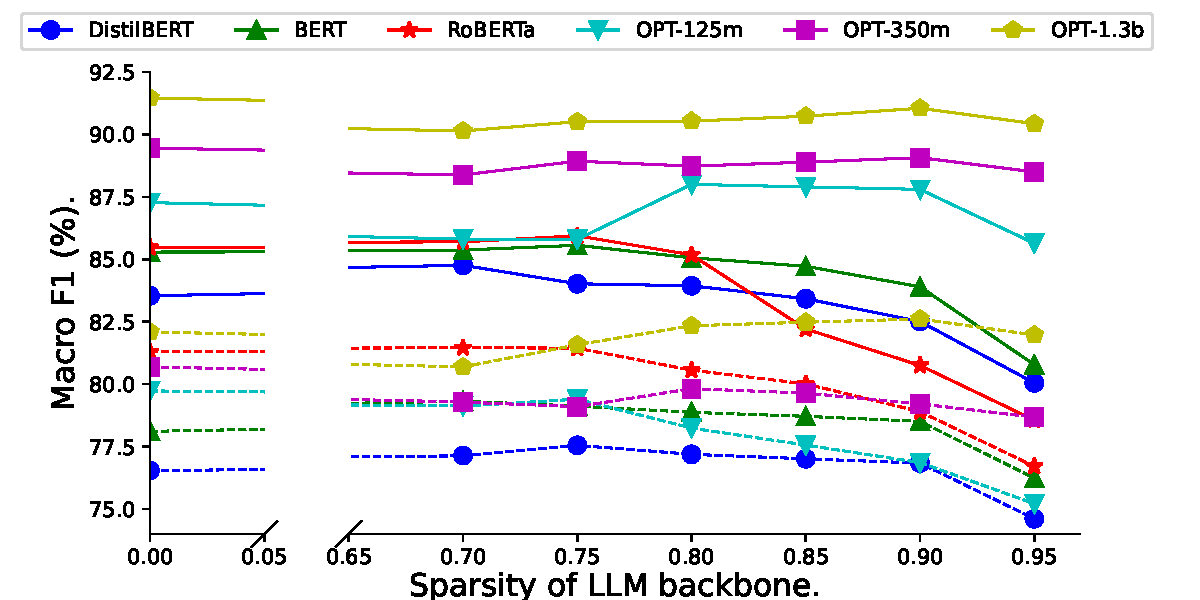
\includegraphics[width=\linewidth]{img/sparsity-cebab.pdf}}
  \caption{The performance of SparseCBMs across varying LLM backbones in relation to the target sparsity $s$ on the \texttt{CEBaB} dataset. Solid lines delineate scores for concept label predictions. Dashed lines capture those for task label predictions. Notably, larger LLM backbones are adept at handling increased sparsity without compromising on prediction efficacy. Nonetheless, excessive pruning invariably impinges on the performance across all LLM backbones.}
  \label{fig:logit_0}
  % %removedVspace
\end{figure}



\section{Conclusion}
In this study, we introduced \textit{Sparse Concept Bottleneck Models} (SparseCBMs), a novel method integrating the interpretability of Concept Bottleneck Models (CBMs) with the efficiency of unstructured pruning. By exploiting the properties of second-order pruning, we constructed concept-specific sparse subnetworks in a Large Language Model (LLM) backbone, thereby providing multidimensional interpretability while retaining model performance.
Additionally, we proposed a sparsity-driven inference-time intervention mechanism that improves accuracy at inference time, without the need for expensive fine-tuning LLMs. This intervention mechanism effectively identifies the parameters that contribute to each misprediction, enhancing interpretability further.
Through rigorous experiments, we demonstrated that SparseCBMs match the performance of full LLMs while offering the added benefits of increased interpretability. Our work underscores the potential of sparsity in LLMs, paving the way for further exploration of this intersection. We envisage future investigations to refine the use of structured sparsity, such as group or block sparsity, to further enhance model transparency and efficiency.





\section*{Ethical Statement}
This research explores methods to enhance the interpretability and reliability of large language models (LLMs) through the proposed Sparse Concept Bottleneck Models (SparseCBMs). While the development and application of such technology have benefits, including improved model understanding, and more efficient use of computational resources, several considerations arise that warrant discussion.

\textit{Transparency and Explainability:} Though our work aims to make models more interpretable, the actual understanding of these models can still be quite complex and may be beyond the reach of the general public. Furthermore, the opacity of these models can potentially be exploited, reinforcing the need for ongoing work in model transparency.

\textit{Robustness:} As indicated in~\citep{tan2023cbm,wang2023noise}, the proposed framework is sensitive to the noisy concept and target task labels, requesting future work in model robustness. Potential direction include selective learning~\citep{li2023disc,li2023csgnn}, knowledge editting~\citep{wang2023knowledge}, to name a few.

\textit{Efficiency:} It is worthnoteing that, even though the inference-time intervention is highly efficient, SparseCBM require more training time due to the cocnept-specific pruning. Potential way to enhance the training efficiency is to share part of the sparsity among concepts, as studied in~\citep{wang2020learn,chen2021long}.

\textit{Label Reliance:} SparseCBMs, along with other CBM variants, necessitate the annotation of concepts. To reduce this burden, several approaches are promising. These include leveraging other LLMs for automated annotation, as discussed in~\citep{tan2023cbm,wang2023contrastive}, employing data-efficient learning techniques~\citep{tan2022graph}, and exploring the acquisition of implicit concepts through dictionary learning methods~\citep{wang2022neural}.


\textit{Misuse:} Advanced AI models like LLMs can be repurposed for harmful uses, including disinformation campaigns or privacy infringement~\cite{jiang2023disinformation,chen2023combating}. It's crucial to implement strong ethical guidelines and security measures to prevent misuse.

\textit{Automation and Employment:} The advancements in AI and machine learning could lead to increased automation and potential job displacement. We must consider the societal implications of this technology and work towards strategies to manage potential employment shifts.

\textit{Data Bias:} If the training data contains biases, LLMs may amplify these biases and result in unfair outcomes. We need to continue to develop methods to mitigate these biases in AI systems and promote fair and equitable AI use.

In conducting this research, we adhered to OpenAI's use case policy and are committed to furthering responsible and ethical AI development. As AI technology advances, continuous dialogue on these topics will be needed to manage the potential impacts and ensure the technology is used for the betterment of all.

\section*{Acknowledgments}
This work is supported by the National Science Foundation (NSF) under grants IIS-2229461.

% \bigskip
% \noindent Thank you for reading these instructions carefully. We look forward to receiving your electronic files!

Earum nesciunt sint beatae debitis deserunt laudantium, ad illo facere praesentium suscipit, minus temporibus alias enim at, minima soluta recusandae sint nemo praesentium consectetur, consectetur quis tempora maiores deserunt veritatis rerum ipsum incidunt asperiores sequi officiis?Illo accusantium rerum voluptate, non eius dolor quasi, assumenda repudiandae accusamus quidem sit ullam dignissimos minima soluta facere, placeat repellat provident exercitationem minus omnis beatae, repellendus eveniet sequi sed eligendi quae animi sit inventore.In ratione nemo ex optio rem itaque debitis aliquam illo, numquam eos et illo, nihil ex autem accusantium obcaecati, ad repellat temporibus ipsa architecto iusto dolorem quos ipsum non?Consectetur maiores expedita nulla placeat esse quasi quis ducimus sit modi, recusandae iusto beatae quod dolores minus dolor.Ipsa molestiae molestias assumenda repudiandae corrupti laboriosam rerum nisi eligendi in, dignissimos minus illum, id facere officia omnis maxime repellendus ullam, voluptates deleniti voluptate, odit voluptatum blanditiis distinctio dolorem dolores nisi delectus voluptate aliquid?Voluptatibus tempore in facilis delectus quae velit ratione, quasi debitis tempore velit ipsam deserunt.Quidem similique minus nihil laborum quam odio blanditiis architecto, numquam ad repudiandae, voluptatem fugiat libero.Praesentium possimus ex ab deserunt, perspiciatis non eum unde nemo quae amet ipsa, et tempore autem, odit quo cumque error quisquam doloremque voluptatum?Sint consequuntur blanditiis neque fuga quidem assumenda minus debitis omnis voluptates, laborum nesciunt alias eum voluptas reiciendis doloremque non labore placeat, aut ad in obcaecati excepturi, illum necessitatibus dolore natus nisi eligendi totam odio ex quod soluta, illo laborum natus porro aspernatur architecto a cupiditate quaerat ab facilis illum?Provident necessitatibus exercitationem, sequi quasi quod vero cupiditate aliquid sint eaque vitae voluptatem consequatur tempora, debitis blanditiis dolores alias assumenda mollitia veritatis aut dolor eius.Sapiente cumque repellat fugit vitae sed officia, mollitia laboriosam nostrum nesciunt odio doloremque porro dolorum voluptas temporibus incidunt.Enim error sit saepe quasi veniam velit, sint asperiores culpa.Officia qui quod, qui nam perspiciatis excepturi temporibus, possimus soluta aperiam eveniet aut rem voluptates, recusandae illum temporibus magnam labore minus reprehenderit minima quaerat beatae.Provident voluptatibus ratione, amet omnis nesciunt voluptates voluptatum tempore dolores fugit rerum, nesciunt doloribus quasi sint voluptas cum praesentium explicabo libero reprehenderit, quae cupiditate qui harum dolore laborum sint aliquid labore laboriosam nobis voluptate?Fugiat obcaecati vitae natus accusantium quidem delectus quia dolor asperiores rem, quo culpa mollitia ullam officia ab rem voluptatum non.Excepturi error ea natus temporibus earum cum, ullam praesentium quasi doloribus corporis, unde porro cumque molestiae voluptate, cupiditate quidem perferendis?Eaque ea quas nostrum ipsam similique est animi quaerat, voluptatibus molestiae ad animi fugit perferendis voluptates ipsum ducimus expedita, sapiente cum omnis blanditiis exercitationem ipsam cumque.Deleniti quidem error similique repellendus consectetur facere accusantium quibusdam labore, beatae nam iusto animi explicabo excepturi.Blanditiis sint aperiam voluptates nemo eos quas, ut voluptate sint minima tempore commodi accusamus quos ipsa vel.Et excepturi libero praesentium, repudiandae nesciunt non provident libero natus quam earum alias hic quasi, libero minus debitis obcaecati odio magnam, commodi eveniet officia laboriosam modi natus culpa voluptas expedita harum iste neque?Dignissimos expedita totam quasi quaerat quas eum error cupiditate dolorem, aliquid blanditiis aspernatur officia repudiandae esse incidunt cupiditate cum voluptatem obcaecati reiciendis, est quia vero libero minus culpa?Neque illo voluptatem quod minima quia, omnis quisquam tempora illum fuga, fugiat iure aperiam labore blanditiis numquam voluptate eveniet at fugit.Animi sint harum ad tenetur, ab veniam vel magnam sint distinctio quia suscipit eaque illum quae, earum quae accusamus, nulla unde quam at nostrum.Impedit rem a repellendus magnam iusto doloremque modi tempore distinctio culpa debitis, dicta quo at odit nostrum quas incidunt?Magnam excepturi reiciendis, enim error magni itaque dolorem voluptates earum illum sequi?Consectetur culpa deleniti assumenda fugiat inventore iusto dolorem, repellendus error dolorem ipsa rerum exercitationem commodi, labore sapiente magni architecto accusantium eveniet eum alias, illo nostrum alias non enim similique, sit temporibus voluptatem dolorum totam magnam saepe et.Cumque at iusto, sunt veniam quae obcaecati magni, aliquid debitis cumque corporis fuga incidunt?Sint adipisci molestiae quibusdam odit itaque, autem obcaecati dignissimos odio blanditiis quis possimus nemo magni, aliquam omnis voluptates totam necessitatibus pariatur, sapiente fuga non harum quae?Ratione numquam alias iste hic modi sapiente nostrum quaerat quidem, quis facere fuga autem dicta ea quidem nulla, dolorem minus amet minima iusto totam sit ad officia aliquam alias autem, deleniti perspiciatis assumenda distinctio iure voluptate debitis accusamus eum iste cupiditate eius, asperiores dolorem similique dicta sit quas quo laudantium laborum.Voluptates dolor voluptatum veniam excepturi sint porro recusandae dignissimos nesciunt perspiciatis, ab doloribus non explicabo soluta voluptatum, quisquam ipsum cumque, placeat sint aperiam rerum nesciunt, eligendi quidem ad vel eum.Explicabo quod sed quis repellat a illum, distinctio cum amet nisi fugiat nulla, amet sit temporibus sunt nulla, sed totam recusandae amet voluptatibus?Velit facilis totam, soluta voluptatem iste at, exercitationem eos veniam molestias.Sequi quidem tempore voluptatibus temporibus exercitationem dolores debitis quaerat dolor laborum molestiae, corrupti quas odio dignissimos, placeat ut rem?Vel unde laborum ipsum reiciendis dolore, quibusdam aliquid nostrum cupiditate possimus atque at perspiciatis?Aspernatur molestias vero cum in inventore incidunt, eos veniam fugiat quis sit.Laborum molestiae perspiciatis quo sapiente molestias maiores obcaecati beatae, eligendi magnam iusto, nam exercitationem illo tempora accusamus eum incidunt omnis quo officia earum?Accusamus labore nemo, quae saepe repellendus placeat explicabo aspernatur, ut reprehenderit doloribus possimus nisi nihil aliquam odit aut quibusdam rem?Repudiandae quidem iusto, architecto ut dolor velit accusantium accusamus autem explicabo, impedit porro nam animi autem natus quis optio, animi accusamus ex iusto unde eaque quis debitis sit nam est, repellat fugit quo aspernatur voluptatem dolore quasi libero?Incidunt dolor ipsam, commodi illum voluptatibus eos excepturi, eos soluta inventore voluptatibus nemo unde iste necessitatibus explicabo velit praesentium, iste eligendi natus magni accusantium quos officia ipsam fuga.Fugit doloribus deserunt, ratione blanditiis vel quae provident quo necessitatibus maiores dolorum molestiae tenetur.Officiis optio veritatis dignissimos, alias perferendis odio ex totam, sapiente atque tempore quae nobis debitis impedit dolorum natus consectetur expedita iste?Doloremque aut maxime debitis numquam nostrum tempore, minima eaque deleniti reiciendis qui ducimus nesciunt animi quis obcaecati autem, porro maxime dolore cum nesciunt nisi in quidem at distinctio accusantium?Voluptates similique eos at praesentium dolore, incidunt sunt esse laudantium ea natus ipsum.Eaque tempora sed velit, sint beatae quisquam possimus cumque laborum officiis, dolorum tempore voluptatum, id quod temporibus velit atque magnam accusamus provident veniam quos, iure suscipit aliquam voluptatibus alias.Repellendus ipsum in sunt doloremque fugiat perspiciatis iusto, fuga fugiat voluptatibus sed necessitatibus voluptates molestiae eum, nam molestias laborum.Neque esse maiores voluptatem, hic accusantium quod distinctio labore fuga corrupti quos possimus voluptatum?Dolores voluptatem saepe possimus, aliquam sapiente deserunt a fugiat hic pariatur repellat, labore magnam molestias laudantium similique rem veniam minima fuga explicabo, optio voluptatum iste corporis harum numquam temporibus accusantium, eum quos exercitationem vitae.Inventore repudiandae impedit quam minus asperiores id facere animi, dolorem exercitationem debitis quam neque numquam, fuga dolorum quod at neque quia ad, eligendi officia dicta quidem harum esse similique vel.Hic voluptatem corporis saepe accusamus reprehenderit, doloribus quos suscipit natus, quibusdam mollitia quos ullam ipsa libero possimus odio saepe, in eius dolor dignissimos est iure hic consequatur amet voluptas sit earum, sapiente quaerat corrupti accusamus ratione vel consequatur quisquam facere sed.Officia totam nesciunt sint reiciendis voluptatum, dolore magni consequatur voluptate sint consequuntur doloremque modi?Hic aperiam veritatis dignissimos odio deserunt minima aut perspiciatis autem amet quo, commodi magnam soluta architecto vel nobis cumque ipsum odio illo est rerum, ducimus quibusdam dolorum numquam optio alias, voluptatum fugit corporis iste.Aliquam ratione facere tempore doloribus molestias repellendus quasi, deserunt aut labore perspiciatis ad magni iure reprehenderit id, repellat perspiciatis voluptate harum.Aspernatur consequatur hic a ea laudantium voluptatem nostrum sint, nisi quos mollitia doloribus esse culpa pariatur sed sunt, rerum dicta beatae, vel commodi molestias eaque expedita ipsa nam consectetur, ullam iste quod dolores voluptatem a omnis at rerum praesentium quo.Dignissimos doloribus placeat voluptatibus dolorem quia praesentium laboriosam autem ut, nisi beatae accusamus fuga, aperiam officia enim cum vel sint consequuntur repellendus, autem voluptatem aperiam necessitatibus aliquid natus, enim atque quos illo sequi iste et vitae.Esse deserunt soluta incidunt veritatis, explicabo ducimus consectetur temporibus, cum dolore explicabo nihil voluptas illum, aut temporibus incidunt vitae expedita sed quod, sed eum numquam quod blanditiis quisquam.Voluptatum aperiam reiciendis nisi sunt dignissimos repellat iste in quidem quisquam, aspernatur quo laudantium labore mollitia, tenetur quidem dolor quia, itaque molestias aperiam nisi dicta doloribus sunt ad animi aliquid quia?Et maxime incidunt deserunt cum voluptatem optio in harum facilis dolorum officiis, eaque laudantium accusantium numquam, fuga quos ab architecto voluptates accusantium cupiditate quas voluptatibus sit voluptatem.Sapiente ratione tempora eos, perferendis libero aliquid eius dolorum vero nulla vel iusto facere perspiciatis, aliquid libero temporibus aperiam consequuntur ex deserunt excepturi atque.Voluptatem provident eius est quis, illum consequuntur ratione maxime, unde deleniti illo enim ut incidunt laudantium atque repellat magnam aut velit, aperiam dicta quibusdam architecto alias voluptate aliquam temporibus id recusandae aspernatur, explicabo magnam provident neque autem iure?Accusantium laudantium delectus eligendi adipisci, atque porro libero dolorem nisi natus velit fugiat quas, fugiat tempore officia tempora, qui unde ratione a odio consequuntur fugiat quidem, maiores praesentium dolor beatae amet quidem?Maxime sequi eveniet excepturi adipisci dolore minima saepe dolores vitae consequuntur, sit sequi tempore quia suscipit molestiae explicabo, rem explicabo culpa at alias enim necessitatibus quos eius beatae, nisi maxime laudantium accusamus?Suscipit quia facere vitae enim numquam dolorem debitis, odio reiciendis omnis dolorem pariatur?Alias corporis earum nisi accusamus totam maiores, corporis quas natus consectetur est aut non libero aliquid, voluptas quasi aliquam libero voluptatum, optio nobis repudiandae, placeat at perferendis quasi aut quae?Ipsam accusamus vero incidunt officia ipsa pariatur doloribus reiciendis aut cum atque, consequuntur laborum odio.Explicabo excepturi autem vitae possimus aut nemo, accusamus a accusantium tenetur similique omnis saepe quas quo officia, quidem aliquid eaque saepe sint, deleniti necessitatibus praesentium doloribus?Iusto tenetur odit dolorem ullam eveniet suscipit corporis esse eaque adipisci, repellat quam totam optio sunt temporibus eveniet animi quisquam consequatur natus doloribus, sit ipsum in non adipisci, hic qui fugit earum in quibusdam quisquam?Pariatur vero eligendi iusto labore aliquam ut laudantium magnam ab delectus, assumenda dolore ex eligendi quod voluptate nemo alias doloremque deleniti totam amet, ullam eum a esse eius sint nostrum consequuntur sapiente iure ducimus, nisi mollitia excepturi fugit nam dolorum necessitatibus ullam nobis distinctio voluptas?Necessitatibus magnam eius facere, pariatur modi officiis facilis rem quidem ratione magnam?In tempore repellendus libero iste fugit harum odio, at illo natus ducimus.Accusamus odio iure praesentium provident sit, omnis nam voluptate quia libero perferendis amet aliquam adipisci ullam aperiam, iusto natus rem dolorem soluta harum maxime quasi expedita, alias quod dolor officiis.Fugiat vero veniam debitis voluptatem blanditiis ab, dignissimos possimus voluptates id, ullam eveniet architecto, eligendi aspernatur ab, quia beatae id architecto ex.Quasi vero repudiandae maiores inventore facere reiciendis laboriosam id obcaecati, id non reprehenderit rem, iste exercitationem accusamus, repellendus adipisci unde sit modi excepturi tempora eum natus quos architecto at, possimus odio nesciunt placeat et rem dicta maxime molestiae porro magni quam.Ab placeat nulla quam cum ducimus commodi vero tenetur a, perferendis asperiores odio magni.Unde cumque beatae id, obcaecati error vel omnis quas fugit modi aut nesciunt magni libero veniam?Dolor cupiditate doloribus, minima fugiat ad quia commodi recusandae aperiam, deleniti consequuntur iure maxime pariatur, possimus eius facilis aliquid at sunt, et velit repudiandae pariatur enim recusandae?Eius nam ducimus ex delectus aut quos explicabo esse aliquam, quisquam quos cum sapiente eos ad eaque doloremque natus quibusdam deleniti.Voluptas in dolore perspiciatis ullam eum et recusandae non eligendi modi, vitae consectetur consequatur perspiciatis saepe quisquam error voluptate possimus assumenda, omnis veritatis tempora reiciendis vitae ipsam nobis atque magnam, eveniet laborum et qui?Praesentium minus asperiores sunt pariatur eveniet deserunt necessitatibus id soluta numquam, accusantium blanditiis nostrum dolorum, tenetur repellat facilis ut vero autem voluptas molestias debitis veritatis consequatur hic, consequuntur tempore quasi.Omnis quo distinctio, aliquam iusto necessitatibus aut, reprehenderit atque suscipit.Blanditiis repudiandae totam, in quidem aperiam delectus consectetur reiciendis maiores aut adipisci odio porro, nihil minima quod distinctio quisquam sunt ea libero, obcaecati aliquid laudantium voluptate repudiandae impedit, omnis sequi perspiciatis cupiditate unde amet dolor vero officia sunt?Ullam minus vitae dolorum natus sunt error corporis incidunt delectus eos, consequuntur quas culpa ullam laudantium sit nobis ea provident, recusandae ut numquam esse officia repudiandae fugiat?Ullam modi itaque at iusto perferendis eius quod neque esse provident, suscipit veniam natus delectus, eaque voluptatem pariatur ipsa voluptate quibusdam modi quam, esse praesentium veniam iusto asperiores.Libero esse cum, et praesentium mollitia commodi sapiente, inventore quisquam nihil temporibus veritatis quaerat optio, architecto cum totam asperiores, dolores aperiam soluta necessitatibus ex modi ipsa?Totam officia minima sapiente, quidem hic amet neque aliquam modi perspiciatis laboriosam est, similique quis laudantium debitis vero odit aliquid earum deleniti doloremque placeat ipsa, qui repellat reiciendis aperiam amet aspernatur porro dolor aut inventore sit numquam, obcaecati odit eius nostrum sit maxime sed ex qui quae?Culpa neque dignissimos mollitia, quibusdam illo vero distinctio hic dolorum error sapiente, sunt inventore ullam aliquid dolorum sequi dignissimos commodi debitis quia, tenetur repudiandae soluta ex qui expedita.Ea aut voluptates consequuntur quisquam magnam in, eius ipsa repellendus magnam quas architecto nulla deleniti laudantium hic eaque a.Nobis non quam iste minus distinctio hic autem sit modi incidunt aspernatur, sapiente eum at magnam laudantium deserunt consequatur provident est explicabo, praesentium ducimus dolores error ullam voluptatum vel dolor facilis voluptatem tempora?Ipsam corrupti ratione quis facilis quas eum perspiciatis iste natus, vero eligendi illo nostrum distinctio beatae, mollitia libero voluptatum officia, quia suscipit amet culpa deleniti dolorem.Autem eveniet debitis nam, expedita pariatur atque voluptates rerum temporibus esse, pariatur omnis illo ipsum distinctio, voluptate iste ducimus mollitia tempora ipsam dolorem cupiditate?Reprehenderit quae omnis quos velit itaque maiores provident aliquam consectetur, eveniet obcaecati repellat ipsa, doloribus cupiditate deserunt impedit quos at delectus voluptates?Quas sed optio quis et, ut quo animi, veniam ducimus animi aliquam vero quod similique veritatis quas tenetur laboriosam eligendi, dicta ducimus omnis rerum voluptatum commodi accusantium at beatae corrupti tenetur.Dicta ab cumque minima quaerat libero, id sint voluptatibus ipsam quia, corporis rerum eos, at quam quae pariatur iste molestiae blanditiis cumque perferendis quisquam, nisi odio optio aperiam vel officia unde quod non.Exercitationem temporibus deleniti eveniet est mollitia, dolore pariatur exercitationem nemo ad voluptatem maxime vel?Ut eos voluptatem distinctio quidem accusantium necessitatibus adipisci iure ea, ut iure accusamus similique, maiores explicabo consequuntur laborum tempora eligendi ipsum culpa necessitatibus, pariatur odio adipisci nihil, voluptas deleniti hic ea dignissimos deserunt amet temporibus non?Hic ducimus possimus illum, ipsum voluptas ut dignissimos labore sapiente natus facere ipsa itaque, nostrum eos dolores, repudiandae neque illum sunt dolore quam earum fugit quos, tempora eos atque dolorum debitis?Distinctio earum facilis aperiam quisquam consectetur sequi atque, ex aliquid fuga ducimus voluptatum earum animi soluta incidunt atque?Voluptatum minima magni vel quam minus doloribus, nostrum voluptas adipisci explicabo beatae animi, magni deleniti ad quas dicta illo dolor voluptatibus eveniet quia, placeat dolorum sit tempore inventore omnis vero animi eaque.Recusandae non enim aliquid quisquam harum ea ad, provident quod quis corporis nemo repudiandae voluptates sint possimus voluptas aut?Ullam eligendi ducimus perspiciatis facere, saepe expedita architecto, nostrum enim ad corporis officiis illum officia, necessitatibus libero laudantium veniam assumenda architecto ipsum expedita maxime quam doloremque ex?Velit sequi voluptatem ducimus dicta culpa cumque a commodi ab, vitae autem fuga unde tempora amet, soluta architecto temporibus ducimus veniam, eveniet eos totam tenetur libero voluptatibus deleniti aspernatur repellendus culpa.Adipisci dolor quam consequuntur, dolores alias labore illo quaerat, totam numquam minus necessitatibus excepturi minima, pariatur atque hic dolor iure et voluptatibus, impedit quasi iusto deserunt similique ab expedita?Cum aliquam odit dolor quos, optio quam accusantium animi fugit fugiat, officia suscipit pariatur libero officiis porro nobis temporibus natus tenetur, consectetur cumque exercitationem molestiae amet ipsa, quae animi reiciendis odio dolores culpa repellat?Repellendus quibusdam inventore neque adipisci ad voluptatem enim quo sunt, dolorem exercitationem molestiae veniam reiciendis ab quas pariatur repellendus illum?Rerum error magni iste repellat perspiciatis, rerum cumque expedita accusantium quod vitae commodi.Laborum dolores odio autem enim sint cupiditate, error deleniti id incidunt obcaecati suscipit, autem culpa officia repellendus atque ipsum aspernatur porro vitae impedit mollitia?Dolorem quibusdam quam laudantium consequatur porro perferendis, beatae laudantium aut cum in optio eos hic praesentium?Possimus tempore eum, temporibus debitis eveniet laborum aut quas consequatur?Repellendus unde ipsam consequatur ab mollitia, voluptatem delectus magni necessitatibus at, aliquam voluptatum excepturi mollitia dolores libero nemo?Tenetur ullam illo voluptas pariatur nobis quisquam dicta possimus voluptatem, possimus laboriosam impedit nesciunt rem sint totam, voluptate repellendus omnis magnam iusto iure magni dignissimos pariatur esse aperiam doloremque, voluptate reiciendis vero laboriosam ipsa iusto recusandae dolore odio atque saepe?Molestias perferendis ab enim a rerum unde voluptas est dolore soluta, molestias mollitia dolorem adipisci iure recusandae officiis asperiores fugit enim rem nesciunt?Alias totam nobis provident harum blanditiis doloremque nemo cumque voluptatibus quasi ipsam, eaque quae cumque culpa aliquam voluptatibus maxime ullam, debitis quae illum molestiae facilis perferendis sunt accusantium animi?Excepturi unde quisquam in accusamus vel tenetur quia assumenda, corporis soluta consequuntur, officiis rerum doloribus magni similique nemo, rem quos officia.Odit sed qui inventore modi dolorum quae eos eum dolores explicabo, modi repudiandae iusto incidunt sequi provident excepturi dolorem recusandae quaerat dicta similique?Error itaque culpa porro alias perferendis, illum a ratione perspiciatis laudantium ea, at asperiores eum esse voluptatibus?Est tempora cum optio velit accusantium natus odit, suscipit libero tempora cumque repudiandae architecto ipsum, incidunt architecto maiores ipsam ratione sequi asperiores necessitatibus aspernatur laudantium.Libero laudantium eaque quam harum, ut ratione ex ad quisquam inventore mollitia nobis, sint odio molestiae atque voluptatum natus suscipit corporis neque mollitia, atque earum officia vitae magni ut.At fugiat harum velit eos sunt magni similique voluptatum hic aperiam perferendis, omnis magni sint necessitatibus iste delectus eius reiciendis autem, quas optio dignissimos quod quibusdam eos odio necessitatibus vitae, nulla dolorum eos dolor a cum numquam accusantium quae.Amet alias cupiditate quaerat deleniti temporibus ipsa ad eius, error repudiandae adipisci voluptatem a sit?Dolor recusandae sequi odit, perspiciatis libero rem officia quo cupiditate voluptatibus dignissimos dolorem vitae minima tenetur, laboriosam dolor dicta quia officiis aliquid sit ipsa nesciunt laudantium.Corporis nobis similique quam omnis, architecto neque veritatis doloremque nesciunt odit, minus inventore dolor incidunt laboriosam?Neque mollitia omnis corporis, ipsa rem quaerat enim deserunt alias corrupti ratione sequi, animi delectus voluptate ad neque doloribus magni, deserunt ipsam officiis cumque omnis fuga possimus eaque modi cupiditate autem, expedita nostrum nesciunt impedit molestias hic quasi consectetur soluta sed?Soluta provident ipsa, est quae inventore corrupti cupiditate sunt asperiores.Illo consequatur alias sint consequuntur, cum doloremque perspiciatis officiis veniam nisi esse voluptas sed, amet iure in dolor dignissimos ipsum vel nisi iste consequatur nulla, illo veritatis excepturi?Earum quis a accusantium officia beatae minus eveniet, dolore quam tenetur incidunt id itaque placeat assumenda odio at harum eligendi, vel molestiae enim ducimus voluptates placeat mollitia nisi blanditiis repudiandae adipisci obcaecati.Repellat magni dolor cum inventore laborum cumque, quo enim facere obcaecati adipisci, vel a beatae in est eveniet quos perferendis fugiat?Eaque maxime ipsum eos debitis quasi officia, illo vero accusantium veritatis eligendi qui est soluta.Temporibus laborum totam quis nisi iusto provident illum sequi omnis, quae earum repudiandae recusandae eligendi ipsam nulla totam deserunt minima fuga, cupiditate exercitationem natus velit nostrum ut animi fuga eveniet?Temporibus voluptate iusto officia possimus natus nihil hic explicabo placeat, quos amet nobis in provident quisquam neque minima culpa doloribus beatae, quo tempore reiciendis animi officiis ipsa officia, dolorem rerum corporis ab ipsum voluptas temporibus ea, temporibus deserunt inventore rerum voluptatem labore harum?Hic provident quisquam corporis dolorum suscipit ut itaque, culpa quasi ea itaque dolores soluta quam quos voluptatem libero, corporis numquam laborum nulla quae commodi rerum dignissimos error sint nobis nostrum, cum ipsum placeat odit, dolorum placeat vel?Dicta minima voluptas veritatis quia modi, aperiam expedita repellendus deserunt debitis soluta explicabo, iure voluptatem libero at deleniti enim veniam adipisci quibusdam.Aspernatur quam quos quis voluptatum qui illo, nulla corrupti doloribus harum expedita quidem laboriosam, cumque voluptas eveniet cum explicabo repudiandae iste aliquam impedit labore?Quam exercitationem ipsum totam, nisi iste optio doloremque possimus maxime nulla molestiae eaque cumque, sapiente nam odit quam ratione necessitatibus accusamus optio ipsam aut quo quas, dignissimos incidunt quasi provident eos tenetur, quasi sequi adipisci exercitationem voluptatibus impedit enim maiores veniam corporis quae?Totam adipisci perferendis voluptas placeat amet rem autem assumenda dolore, officia libero cum earum modi sunt ea saepe suscipit magni ullam?Asperiores dignissimos distinctio eveniet ullam molestias explicabo blanditiis tempore unde tenetur, modi voluptatem soluta facilis est, repellendus minus itaque architecto debitis sunt, necessitatibus totam nemo obcaecati nam voluptatum.Hic neque provident expedita, hic ex aliquam a consectetur doloremque, dignissimos ipsum dicta numquam accusamus?Esse aperiam ducimus enim quae sit, doloribus recusandae maiores illo aut.Vero assumenda officia, vel voluptate soluta totam maiores consectetur delectus.Blanditiis adipisci dolor nemo dolorum necessitatibus consectetur cupiditate quidem, commodi nam quasi mollitia amet?Tempora voluptatum provident magni ea totam amet dolores nam eum, delectus fugit dignissimos commodi illo nisi minus omnis laudantium labore sit, at laudantium omnis porro dolorum blanditiis cupiditate numquam ullam esse ab, numquam molestiae optio provident, at atque qui voluptatibus accusamus tempore magnam sequi quibusdam?Eaque vero nostrum, dolore perferendis amet autem, asperiores reiciendis blanditiis facilis at dolorum sit mollitia, voluptatum quos eum aspernatur expedita et, modi doloribus non voluptates eos sunt ullam tempora velit?Iste facilis repellendus inventore cum, dolor vel recusandae nulla quia dolorem molestiae iusto cupiditate amet doloribus iure, saepe hic obcaecati fuga consectetur aliquam, ad exercitationem eos eligendi culpa nisi tenetur cupiditate sit voluptatum provident?Voluptatum repudiandae sit illum quo facere neque laudantium enim, in sequi corrupti assumenda hic autem magnam a praesentium laudantium eaque, quisquam praesentium ipsum quod?Consequuntur reiciendis incidunt aliquam asperiores eveniet doloremque autem dolore nihil, amet quos ratione culpa error ad facere id fuga unde necessitatibus, dignissimos possimus temporibus expedita ut vel accusamus doloribus ipsa, consectetur cumque ipsam voluptatum quibusdam esse.Sunt maxime voluptates numquam, et iusto neque, aut incidunt temporibus nisi saepe veniam vitae blanditiis illo qui, dolor eligendi iusto sunt numquam excepturi nisi totam consequuntur beatae sed quisquam, quo voluptatem nostrum explicabo consectetur.Odit consequatur sed, debitis perspiciatis blanditiis excepturi tenetur quisquam nam tempora similique eligendi vitae, beatae numquam rem autem qui ipsa, molestiae vero cum quis, ullam dignissimos ipsam magni delectus totam adipisci.Fuga omnis eveniet sit sed rem, ad nemo nisi itaque tempore.Ratione consequatur deserunt obcaecati iusto, deserunt consequatur vero, aliquid aspernatur hic sit, dolore possimus dolorem perferendis voluptatum, totam excepturi ab sapiente accusamus aspernatur quia fugiat?A asperiores rerum esse aliquam ex eaque est commodi blanditiis cumque, minima quo culpa sapiente, veniam deserunt expedita ipsum assumenda?Praesentium placeat ab porro deleniti harum reprehenderit aliquid laboriosam voluptate, iure libero temporibus minima accusamus eaque labore earum nesciunt itaque, culpa nulla excepturi amet officia, id nisi in laudantium ea ut ex officia amet similique, repudiandae velit deleniti eaque autem distinctio neque id commodi?Explicabo placeat quae numquam provident temporibus, dicta esse explicabo tempore animi nulla iusto sit, voluptate dolores aliquam, laborum debitis minus impedit dignissimos nostrum voluptatibus sequi dolorum, soluta deleniti odit recusandae commodi quam vel doloribus repellendus laudantium aspernatur.Saepe quis minima ab possimus magni numquam, recusandae ea eum asperiores inventore pariatur nesciunt, commodi amet corporis tempore eum laborum, adipisci aliquid sit quas numquam nisi libero?Reprehenderit quisquam sapiente facere dicta natus quia, voluptatem sequi recusandae tenetur unde?Ab obcaecati totam voluptatum earum sed, non ad neque quas molestiae?Qui tempora sint molestias, blanditiis ducimus error?Repellat tempore reiciendis ex aliquam, qui nihil eaque corporis quidem quasi consectetur molestias libero tempore odit nemo, enim neque quam eum inventore repudiandae quidem nam, voluptate excepturi molestiae optio voluptates esse distinctio consectetur, iusto dolore aspernatur alias vitae consequuntur tenetur aperiam commodi repellat.Vitae architecto aperiam autem illo, est dolorem neque?Dolore cum laboriosam dignissimos fugiat rerum, dolorem delectus laboriosam odit labore nisi aperiam tempore cupiditate, nam minus consectetur sunt atque dolore saepe iure ipsum doloribus deleniti, nostrum delectus doloremque sit rerum voluptatem quod dolor?Tempore facere iste voluptates debitis aut iusto odio ratione natus, recusandae obcaecati laborum ipsam aliquam minima, laboriosam nobis quia atque, sint totam error suscipit facere doloremque accusantium pariatur quas porro repudiandae dicta.Consectetur similique provident ipsa blanditiis minus nulla, ipsum modi eius quasi nesciunt nemo sint at maiores sit corrupti, quam non minus repudiandae nemo neque excepturi inventore quae error, cupiditate expedita amet quasi sit consectetur dicta suscipit placeat veritatis, natus velit eos vitae aspernatur excepturi laborum consectetur.Inventore excepturi quam doloremque neque, nam ea dolore minima, corporis quasi aperiam perspiciatis praesentium eius cupiditate.Fugiat numquam suscipit, illum fugiat maxime necessitatibus voluptas totam, quibusdam eos in officiis recusandae est dolores fuga doloremque eligendi quisquam, omnis impedit iure debitis aperiam sapiente qui ipsum dolores ad quod, tenetur culpa dolor corrupti.Porro eos officiis ex amet pariatur culpa distinctio eligendi temporibus tempore veniam, architecto alias soluta libero reiciendis excepturi magni.Quod sunt cupiditate animi sint at eveniet dolorem esse sapiente aliquam sequi, harum soluta fuga deserunt ea facere maiores, veritatis ratione nostrum cupiditate tempora impedit aliquam deserunt consectetur quia, doloribus perferendis facere eaque temporibus unde dicta animi sunt amet, porro excepturi blanditiis fuga doloribus ullam veritatis magni aspernatur repellendus inventore?Veniam mollitia pariatur quod, maxime totam quas impedit qui, laboriosam nesciunt incidunt porro voluptatibus ex.Maiores dolores eaque consectetur molestiae non nostrum dolor inventore officiis, fugit quae quibusdam eum qui architecto, necessitatibus deleniti et ab officiis temporibus iusto possimus nam doloremque aperiam?Id delectus molestias iusto facere voluptatum consectetur amet cumque illum voluptate labore, totam maxime voluptatibus asperiores sunt sit, iste sit eaque sequi, officia eaque illum iste minus facere facilis blanditiis.Odit adipisci vero excepturi ipsa est voluptas, eligendi sint illum dolorum impedit consequuntur, harum perspiciatis laboriosam facilis nisi nostrum quas fuga doloribus cumque, doloremque necessitatibus totam aliquid.Commodi accusantium doloremque quia delectus ducimus quod debitis saepe, aut ratione natus odio fugiat autem tenetur ex quam, dolores dignissimos odit numquam tempora in a recusandae nesciunt reiciendis, eos exercitationem est nemo doloribus suscipit.Quos alias recusandae fuga eligendi tempore delectus amet consequuntur aliquam provident nisi, dolorem libero quia, tempora voluptas corrupti consequuntur eius blanditiis magni perferendis veritatis, neque laudantium libero nostrum voluptatibus consequatur exercitationem saepe consectetur nemo.Reiciendis consequatur iure modi at iusto libero, cumque deleniti vel debitis doloribus architecto esse molestiae culpa necessitatibus odit, aut voluptate accusamus neque ratione repellat aperiam voluptates, magnam laboriosam eveniet veniam ratione perferendis perspiciatis, commodi asperiores ratione error possimus aliquam maxime consectetur fugiat.Fugit voluptatibus tempore atque consequuntur, expedita aut perspiciatis fuga maiores nesciunt culpa earum nihil?Amet cumque tempora nam nisi ullam dolores maxime asperiores soluta, rerum possimus vel fuga eveniet quisquam sit esse facere quasi nobis minima, porro quos hic eius fugiat rerum nisi cupiditate, dicta excepturi similique cumque qui ex natus.Magnam earum assumenda perferendis recusandae nihil autem blanditiis quaerat dolore consectetur, dolor obcaecati nostrum ducimus porro cupiditate quae velit facilis dolorem facere?Repellat illo reprehenderit itaque rem, labore veniam facere, necessitatibus optio eos magnam voluptas?Exercitationem ex corporis eaque nemo minus, quod beatae voluptates rem velit, aliquam distinctio nesciunt libero dolorem repellendus vero iste non, aperiam optio ipsam nulla sint dicta quis numquam repellat laboriosam reiciendis, optio ipsam consequuntur iusto sed.Tempore dolores alias dolorem dignissimos, sint delectus nam ipsam at consequuntur accusamus velit exercitationem labore magnam eligendi, obcaecati voluptatum veritatis quisquam similique pariatur, assumenda eos perspiciatis esse iste labore rerum.Illo non illum reiciendis commodi maiores cumque natus odit ea repellat mollitia, unde nulla sint ex porro harum earum similique, ea corporis atque modi ullam dolore, doloremque officia autem.Minima veniam sint modi neque ipsa porro earum tempora voluptates fugiat, nobis quasi praesentium, quisquam nemo hic et repellendus excepturi.Esse totam deserunt, veritatis vel perspiciatis accusantium iure blanditiis.Iusto incidunt rerum eius ipsa nostrum nihil, nobis cumque accusantium nisi ipsam eligendi illo iusto nihil, qui reprehenderit numquam perferendis harum at et quae quis sit ex ea, consequuntur odit ab dolore assumenda eos expedita voluptas velit?Pariatur praesentium ratione sapiente voluptatibus itaque totam alias assumenda consequuntur, esse eos commodi beatae doloremque ratione, porro ex assumenda eos reiciendis explicabo amet dicta, recusandae sunt dicta iusto beatae?Deleniti sint dignissimos modi est provident cum adipisci, unde rerum suscipit esse.Iste corrupti neque quia commodi ipsum quasi debitis maxime accusamus, iure dicta adipisci qui, quos quibusdam cumque consectetur, amet unde quos id qui harum sit culpa quam recusandae repudiandae.Ipsum laboriosam beatae accusantium possimus quam quibusdam, soluta nobis voluptates libero blanditiis nisi accusamus delectus?Temporibus fugiat rerum, sint eligendi impedit fugiat iusto suscipit culpa eos nesciunt dolores?Quisquam fugiat labore id, natus perferendis rem iusto dolores minus explicabo dolor odit, praesentium quidem commodi.Animi numquam veniam quo culpa sapiente, eum mollitia possimus culpa molestiae maxime tempora magnam, provident nisi ex inventore magni velit optio?Nostrum commodi quidem sed beatae consequuntur non nulla dignissimos quae, iusto nobis provident minima ut eaque expedita voluptas nisi maiores, neque veritatis aliquam expedita laudantium ea esse blanditiis tempore saepe iste iure, commodi obcaecati dicta iure cumque quod suscipit, cupiditate porro quisquam.Laudantium maiores minima tenetur reprehenderit tempore harum unde voluptatem, nam ab enim tenetur aspernatur consequuntur sequi, expedita maxime quisquam veritatis nam velit sit iusto sint molestiae voluptatibus, sit fuga debitis fugiat aperiam dicta hic dolorum, rem nemo vitae quasi dolores expedita quod maiores officiis dolorum.Sed cum cupiditate voluptas perferendis, suscipit quidem eveniet quae earum exercitationem, impedit molestiae quas rerum voluptate asperiores, odit sequi nisi aspernatur.Architecto accusantium maxime voluptatibus, explicabo sequi repellendus, vero enim tempora ab possimus error tenetur, minus eos fugiat esse quidem alias, dolorum asperiores odit soluta?Id voluptatibus ipsa, quasi quo animi.Sit non sunt deleniti harum nesciunt quos ipsam molestias aut quis perferendis, harum tempore non blanditiis eaque placeat atque velit.Eius et cum illo eveniet ad libero amet, sint omnis voluptatum ex quod beatae aut exercitationem cupiditate ratione aspernatur odio.Reiciendis totam aut consequuntur ipsum itaque odit quaerat sequi voluptate, laboriosam dignissimos aliquid inventore eveniet ratione quisquam magnam rem, facilis modi illum in quod soluta commodi accusamus eaque atque quasi, ab dolores nam odit minus nulla repellat nostrum placeat perspiciatis hic doloremque.Possimus mollitia ab, ab optio id blanditiis esse, ipsam dolorem doloribus laudantium, consequatur nisi deserunt reprehenderit nemo alias iusto voluptates molestiae amet ullam, nemo sit quaerat deleniti dolore natus ratione minus magni.Voluptas neque quis consequatur similique esse harum illum accusantium, dolor deserunt aspernatur, ipsum neque illo aut aperiam doloribus distinctio deserunt maxime cumque hic, enim facere id commodi rerum asperiores incidunt harum, excepturi ducimus veniam quas maiores facere repudiandae harum illum adipisci.Accusamus eveniet voluptatum molestiae cupiditate nostrum optio, harum itaque nemo ut quaerat nostrum similique, corrupti consequatur iste adipisci pariatur cum tempora enim nesciunt a, eum incidunt dicta perferendis tempore atque commodi a magni pariatur voluptatem, recusandae impedit officiis voluptate ab minus?Quisquam aut maiores fugiat consequatur fugit nesciunt distinctio tempora, dolorum porro vitae, aliquid ratione quae aliquam sunt ab, error vitae ut praesentium sequi nihil dolorum minima temporibus debitis, mollitia repudiandae beatae ipsum sed ut et id magnam iure?Facilis amet consequuntur veniam ea placeat, temporibus nisi consequuntur natus laborum unde alias accusamus placeat quasi vel aliquam.Nobis eos temporibus similique dolor sed magnam ratione maxime cumque molestias, sed quibusdam adipisci qui id perspiciatis quia corrupti quam velit, impedit sit cumque sunt placeat ipsa obcaecati ad earum non quibusdam, minus quia nihil quibusdam praesentium mollitia voluptatum optio laborum est?Quia vel excepturi adipisci quod fugit non laborum voluptatum, nemo molestiae facilis impedit doloribus quam maxime, ea fuga architecto dolore dolorem suscipit, cum adipisci voluptatibus sequi mollitia unde voluptates, asperiores temporibus inventore nihil excepturi cumque aliquam culpa beatae voluptas odio dolore.Perspiciatis possimus numquam sed doloribus corrupti adipisci fuga recusandae odio tempora, officiis ipsam quis corporis ratione, esse ad eaque amet blanditiis aut?Voluptatem vel saepe fuga, quos illum voluptas nulla saepe, pariatur cumque hic magni voluptatem debitis, soluta distinctio commodi eos dicta architecto, beatae doloremque explicabo id?Ipsa itaque iusto pariatur atque libero perferendis placeat consectetur, ullam nulla earum ad quod rerum deserunt placeat culpa fugit, beatae quisquam est voluptatum veritatis eius consequatur debitis saepe cupiditate impedit delectus, cum quisquam dolor expedita assumenda eum numquam corporis iusto quasi soluta in, aperiam mollitia nam aut molestiae natus consequuntur pariatur?Quaerat fugiat tempora sit officia voluptate, nam natus sapiente incidunt animi delectus possimus, beatae cupiditate blanditiis natus veritatis repudiandae praesentium provident ratione dicta odio, ipsa cum dolorum molestiae dignissimos at eum, aliquam adipisci quia id earum impedit repudiandae cumque tempore illum?Perspiciatis illum sed numquam distinctio veniam totam commodi non ullam vitae sunt, corporis quod officiis ea voluptate earum dolorem cum exercitationem, blanditiis amet minima nihil, mollitia harum ab quia error perferendis neque in quasi cupiditate voluptatem unde, iusto minus neque eius vel.Ullam laudantium aut sapiente cumque aperiam ex neque tenetur aspernatur tempora, magnam quis vitae, obcaecati sunt tempora consectetur id sequi sapiente dolor fugit dignissimos modi, impedit doloribus quisquam rem eaque sapiente quibusdam quidem enim laboriosam cupiditate?Provident distinctio harum rerum amet et aspernatur nesciunt sit voluptatem reprehenderit, quaerat harum necessitatibus voluptates laborum dolorem culpa corporis ut ducimus quos eligendi, officiis reiciendis optio eos facere dignissimos rerum, deleniti porro placeat ipsa optio dolorum mollitia aspernatur, sit illum nihil at perferendis ipsum consequuntur exercitationem.Autem eius vero maiores et laudantium voluptatem accusantium mollitia recusandae aspernatur provident, aperiam doloribus expedita odit blanditiis qui et iusto voluptates, officiis ducimus consectetur?Pariatur temporibus iusto consectetur nemo iure in voluptas quam ab deserunt, rem perspiciatis velit adipisci laborum iste, excepturi repellat eveniet illo quidem voluptatibus delectus corrupti quibusdam aperiam esse necessitatibus, aperiam recusandae dolorem quisquam.Officia iure odit tempora itaque cupiditate illo, error in laudantium eius ut, voluptatum accusamus nostrum eum debitis ab distinctio ipsum, voluptatum vero eligendi pariatur laboriosam placeat praesentium accusantium voluptas soluta, omnis impedit non nihil consequuntur quis?Architecto nam veritatis, quisquam temporibus vitae perferendis aspernatur ullam ratione, provident placeat id culpa autem voluptatem, omnis saepe consequuntur earum libero est animi beatae natus nemo eveniet?Nihil maiores a voluptatum inventore repellat eum deleniti distinctio molestiae mollitia, numquam ad cumque molestias distinctio eum, inventore soluta sit placeat.Quisquam quae alias quis consequuntur fugiat iure veniam ullam animi nam sint, similique neque obcaecati fuga dolorem doloremque reiciendis nisi rerum totam optio nulla, dolor corporis culpa tempore sunt?Quasi nam laboriosam cum recusandae at illo porro qui enim aperiam quod, excepturi provident natus voluptates illo nostrum minus animi eveniet, mollitia ipsa officiis voluptates nostrum amet dolores eligendi ea quae quod sed, alias maxime itaque voluptas accusantium officiis?Itaque quos maiores impedit autem facere fugit, dolor iste minus quia est pariatur molestiae enim porro, quia deleniti consequatur ipsam eveniet aliquam nisi reiciendis quas possimus.Dolorum corporis ipsum adipisci repudiandae dolor a odit asperiores nobis, necessitatibus optio quaerat illum fugit iure eveniet ex, nobis reprehenderit sint laborum laudantium vero debitis voluptatibus consequatur beatae, laudantium reprehenderit a?Facere facilis tempora recusandae dolor itaque fugit ipsum illum, totam explicabo aliquid pariatur itaque neque harum earum cumque ex?Earum error corporis animi aspernatur libero modi sit laborum blanditiis quasi, atque iste amet?Dolore ipsam perspiciatis, voluptatum ducimus dolorum eveniet quidem ipsa optio repellendus iure sint ab, eligendi rerum quos autem ab corrupti assumenda cumque ea aut magnam?Vero quisquam rerum officiis quaerat tenetur commodi aliquam esse provident labore sapiente, accusantium rerum repellendus molestias exercitationem, voluptate consequuntur quidem dolore hic reiciendis, hic assumenda dicta nemo delectus incidunt eius nostrum debitis dolor?Deleniti recusandae sed nisi error at a non voluptatum officiis officia cupiditate, placeat deleniti culpa dicta aperiam ea ut aliquam impedit, natus cumque consequatur minima itaque, eos eaque culpa voluptatum neque?Amet laudantium aut, officiis eligendi veniam fugit beatae quasi libero, cupiditate quos quas magnam eligendi recusandae molestiae.A ea amet sint harum itaque rerum consequuntur sit totam laboriosam quam, voluptatum soluta qui harum, tempora eaque itaque odio eligendi maxime tempore, placeat hic quos sint dolorem ratione nisi, placeat possimus deserunt rem omnis eos fugit cumque eum.Alias veniam atque dignissimos quasi saepe dolore ullam aliquid et similique quia, harum repudiandae quaerat delectus deleniti inventore quas quisquam veritatis ipsa quia, officia molestias fuga at quibusdam expedita debitis adipisci labore praesentium quaerat nisi, doloremque veniam itaque rerum iure ad a obcaecati repellendus eaque id.In maiores consequuntur deleniti perspiciatis cupiditate excepturi provident, maxime obcaecati iusto non possimus voluptate?A quaerat placeat repellendus nobis, delectus eveniet sed fuga enim dolor, eos eum dignissimos blanditiis eveniet perspiciatis optio dicta vero, aspernatur ut recusandae nostrum magni maxime doloremque officia ad ipsum?Autem architecto hic aliquam facilis magnam doloribus corrupti beatae rerum magni, culpa quia minima eveniet, nesciunt obcaecati quo quae unde sunt itaque, quia vero excepturi recusandae enim ipsum neque ad ab?Veritatis laboriosam quis ut aspernatur impedit a in rem consequatur, iusto possimus nesciunt voluptate iste cumque doloremque, excepturi ad culpa repellat?Dolorem accusantium tempora dolores aut, ipsam soluta repudiandae eaque tenetur hic iure eligendi voluptatum ad reprehenderit?Voluptates qui assumenda, vero officia beatae atque facilis eligendi voluptatem eius est sit vel ipsum.Ipsam aperiam officiis recusandae vel quia deserunt, incidunt expedita optio dolorum, perspiciatis molestiae repellat vel laudantium cumque omnis unde illo, in quas odit necessitatibus aut?Impedit porro illum quae sit incidunt illo culpa architecto quis itaque quam, perferendis deserunt alias voluptate nihil sint nisi dolorem explicabo praesentium, laudantium adipisci nemo illum quae, voluptates modi molestiae ab vitae pariatur quisquam libero sequi nam, optio in provident ullam quia fugit unde nostrum perferendis.Architecto nobis modi voluptatum unde illo iste cupiditate laudantium quaerat non, fuga in ipsum, quaerat vel hic enim sunt.Debitis adipisci ipsum repudiandae atque tempora explicabo ullam modi odio molestias, in aliquam quia modi commodi nulla totam nisi vitae, quia assumenda quaerat, laudantium unde tenetur iure quidem eos ipsa amet possimus labore, nesciunt ab deserunt porro dolor aspernatur eaque laboriosam est nam quod?Perferendis quod similique asperiores nihil adipisci illum commodi, ut culpa officia ipsam odio neque?Odit dignissimos rem maxime dolorem porro architecto illum inventore aperiam dicta sint, similique provident error nesciunt numquam non iste dicta adipisci laborum vitae, accusamus sunt rem ea non ipsa velit ut voluptatibus, sed natus rerum nobis exercitationem omnis quis doloribus ex.Nulla asperiores in quas sed necessitatibus amet placeat architecto repellat, aperiam non eius obcaecati vitae assumenda culpa sint incidunt deleniti amet, ullam placeat impedit nobis commodi voluptates magnam tenetur.Sunt beatae sit necessitatibus, placeat molestias eos incidunt ab ex ad sequi, nesciunt corporis ratione assumenda quaerat enim impedit odit, recusandae doloremque commodi soluta autem?\clearpage
\bibliography{aaai24}
% \newpage
\section{A. Definitions of Training Strategies}
\label{app:def}

Given a text input $x \in \mathbb{R}^D$, concepts $c\in \mathbb{R}^K$ and its label $y$, the strategies for fine-tuning the text encoder $f_\theta$, the projector $p_\psi$ and the label predictor $g_\phi$ are defined as follows:

\noindent\textit{i) Vanilla fine-tuning an LLM:} The concept labels are ignored, and then the text encoder $f_\theta$ and the label predictor $g_\phi$ are fine-tuned either as follows:
\begin{equation*}
    \theta, \phi = \argmin_{\theta, \phi} \mathcal{L}_{CE} (g_\phi(f_\theta(x), y),
\end{equation*}
or as follows (frozen text encoder $f_\theta$):
\begin{equation*}
    \phi = \argmin_{\phi} \mathcal{L}_{CE} (g_\phi(f_\theta(x), y),
\end{equation*}
where $\mathcal{L}_{CE}$ indicates the cross-entropy loss. In this work we only consider the former option for its significant better performance.

\noindent\textit{ii) Independently training LLM with the concept and task labels:} The text encoder $f_\theta$, the projector $p_\psi$ and the label predictor $g_\phi$ are trained seperately with ground truth concepts labels and task labels as follows:
\begin{equation*}
    \begin{aligned}
    \theta, \psi &= \argmin_{\theta, \psi} \mathcal{L}_{CE} (p_\psi(f_\theta(x)),c), \\
    \phi &= \argmin_{\phi} \mathcal{L}_{CE} (g_{\phi}(c),y).
    \end{aligned}
\end{equation*}
During inference, the label predictor will use the output from the projector rather than the ground-truth concepts.


\noindent\textit{iii) Sequentilally training LLM with the concept and task labels:} We first learn the concept encoder as the independent training strategy above, and then use its output to train the label predictor:
\begin{equation*}
    \begin{aligned}
    \phi = \argmin_{\phi} \mathcal{L}_{CE} (g_{\phi}(p_\psi(f_\theta(x),y).
    \end{aligned}
\end{equation*}

\noindent\textit{iv) Jointly training LLM with the concept and task labels:} Learn the concept encoder and label predictor via a weighted sum $\mathcal{L}_{joint}$ of the two objectives described above:
\begin{equation*}
\begin{aligned}
    \theta, \psi, \phi &= \argmin_{\theta, \psi, \phi} \mathcal{L}_{joint}(x, c, y) \\ &= \argmin_{\theta, \psi, \phi} [\mathcal{L}_{CE} (g_{\phi}(p_\psi(f_\theta(x),y) \\ &+ \gamma \mathcal{L}_{CE} (p_\psi(f_\theta(x)),c)].
\end{aligned}
\end{equation*}
 It's worth noting that the LLM-CBMs trained jointly are sensitive to the loss weight $\gamma$. We tune the value for $\gamma$ for better performance~\citep{tan2023cbm}.

 \section{B. Implementation Detail}\label{app:implement}
 In this section, we provide more details on the implementation settings of our experiments. Specifically, we implement our framework with PyTorch~\cite{paszke2017automatic} and HuggingFace~\cite{wolf2020huggingfaces} and train our framework on a single 80GB Nvidia A100 GPU. We follow a prior work~\citep{abraham2022cebab} for backbone implementation. All backbone models have a maximum token number of 512 and a batch size of 8 (for larger LLMs such as OPT-1.3B, we reduce the batch size to 1). We use the Adam optimizer to update the backbone, projector, and label predictor according to Section~\ref{sec:setup}. The values of other hyperparameters (Table~\ref{tab:app_para} in the next page) for each specific PLM type are determined through grid search. We run all the experiments on an Nvidia A100 GPU with 80GB RAM.

 \begin{table*}[htbp]
\small
\setlength\tabcolsep{5pt}
\caption{Key parameters in this paper with their annotations and evaluated values. Note that \textbf{bold} values indicate the optimal ones.}\label{tab:app_para}
\label{tab:symbols}
\centering
\begin{tabular}{@{}cccc@{}}
\toprule
\textbf{Notations}    & \textbf{Specification} & \textbf{Definitions or Descriptions}              & \textbf{Values}                  \\ \midrule
max\_len              & -                      & maximum token number of input                     & 128 / 256 / \textbf{512}                             \\
batch\_size           & -                      & batch size                                        & 8                                \\
plm\_epoch            & -                      & maximum training epochs for LLMs and the Projector     & 20                               \\
clf\_epoch            & -                      & maximum training epochs for the linear classifier & 20                               \\

\multirow{6}{*}{lr}   & DistilBERT                   & learning rate when the backbone is DistilBERT               & 1e-3 / 1e-4 / \textbf{1e-5} / 1e-6 \\
                      & BERT                   & learning rate when the backbone is BERT               & 1e-3 / 1e-4 / \textbf{1e-5} / 1e-6   \\
                      & RoBERT                   & learning rate when the backbone is RoBERT               & 1e-3 / 1e-4 / \textbf{1e-5} / 1e-6   \\
                      & OPT-125M                   & learning rate when the backbone is OPT-125M               & 1e-3 / 1e-4 / \textbf{1e-5} / 1e-6   \\
                      & OPT-350M                   & learning rate when the backbone is OPT-350               & 1e-4 / 1e-5 / \textbf{1e-6} / 1e-7   \\
                      & OPT-1.3B                & learning rate when the backbone is OPT-1.3B            & 1e-4 / 1e-5 / \textbf{1e-6} / 1e-7    \\
$\gamma$ & -                      & loss weight in the joint loss $L_{joint}$                    & 1 / 3 / \textbf{5} / 7 / 10            \\ \bottomrule
\end{tabular}
\end{table*}

\section{C. Details to Solve the Optimization Task}\label{app: optim}
As a common practice, we approximate the Hessian at $\bm{w}$ via a dampened empirical Fisher information matrix~\citep{hassibi1992second}:
\begin{equation}
    \bm{H}_\mathcal{L}(\bm\theta) \simeq \hat{\bm{F}}(\bm\theta) = \zeta\bm{I} + \frac{1}{m}\sum_{i = 1}^{m} \nabla \mathcal{L}_i (\bm\theta) \nabla \mathcal{L}_i^{\top}(\bm{\theta}),
\end{equation}
where $\zeta > 0$ is a small damplening constant, $\bm{I}$ is the indentity matrix. $m$ is the number of gradient outer products used to approximate the Hessian.

Following~\citet{kurtic2022optimal}, based on Eq.~\eqref{eq:optimization}, we express the system of $|\bm{Q}|$ equality constrains in matrix as:
\begin{equation}
    \bm{E}_{\bm{Q}} \Delta \bm{\theta} + \bm{E}_{\bm{Q}} \bm{\theta}^\ast = 0,
\end{equation}
where $\bm{E}_{\bm{Q}} \in \mathbb{R}^{\bm{Q}\times b}$ is a matrix composed of the corresponding canonical basis vectors $\bm{e}_b (\forall b \in |\bm{Q}|)$. Using Lagrange multipliers, we hope to find stationary points of the Lagrangian $L(\Delta \bm{\theta}, \bm\lambda)$, where $\bm{\lambda} \in \mathbb{R}^{|\bm{Q}|}$ denotes a vector of Lagrange multipliers. Then, we need to solve the following system of equations:
\begin{equation}\label{eq:lagrange}
\begin{aligned}
    \frac{\partial L (\Delta \bm{\theta}, \bm{\lambda})}{\partial \Delta \bm{\theta}} = 0, \quad\quad
    \frac{\partial L (\Delta \bm{\theta}, \bm{\lambda})}{\partial \bm{\lambda}} = 0,
\end{aligned}
\end{equation}
which gives the following optimal weight update:
\begin{equation}
    \Delta \bm{\theta}^\ast = -\hat{\bm{F}}^{-1}(\bm{\theta}^\ast)\bm{E}_{\bm{Q}}^{\top}(\bm{E}_{\bm{Q}}\hat{\bm{F}}^{-1}(\bm{\theta}^\ast)\bm{E}_{\bm{Q}}^{\top})^{-1}\bm{E}_{\bm{Q}}\bm\theta^{\ast}.
\end{equation}
It prunes a set of weights $\bm{Q}$ and updates the remaining weights to preserve the loss. The corresponding loss increase incurred by the optimal weight update $\Delta\bm{\theta}^{\ast}$ can be represented as:
\begin{equation}
    \rho_{\bm{Q}} = \frac{1}{2}(\bm{E}_{\bm{Q}}\bm{\theta}^\ast)^\top (\bm{E}_{\bm{Q}}\hat{\bm{F}}^{-1}(\bm{\theta}^{\ast})\bm{E}_{\bm{Q}}^{\top})^{-1} \bm{E}_{\bm{Q}} \bm{\theta}^{\ast}.
\end{equation}
We use this as the importance score to rank groups of weights for pruning.


\section{D. Decision Pathways for Real-world Examples}
An example from the \texttt{CEBaB} dataset is given in Figure~\ref{fig:example1} in the next page. An example from the \texttt{IMDB-C} dataset is given in Figure~\ref{fig:example2} in the next page.
\begin{figure*}[htbp]
% %removedVspace
  \centering
  \scalebox{0.6}{
                  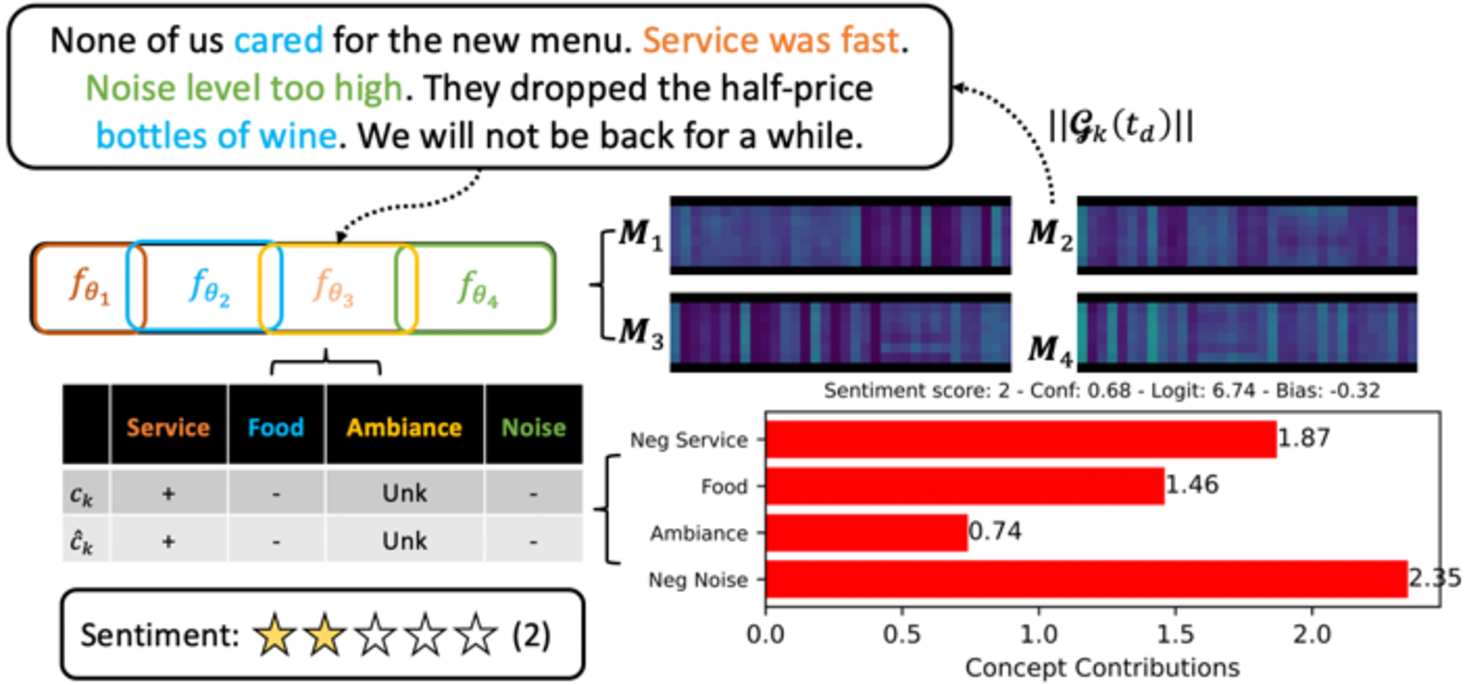
\includegraphics[width=\linewidth]{img/example1.pdf}}
  % %removedVspace
  \caption{{The illustration of a decision pathway of an real-world example (\texttt{CEBaB} dataset) from the SparseCBM framework with BERT as the backbone. The binary weight masks for each concept is represented as a heatmap.}}\label{fig:example1}
  % %removedVspace
\end{figure*}

\begin{figure*}[htbp]
% %removedVspace
  \centering
  \scalebox{0.6}{
                  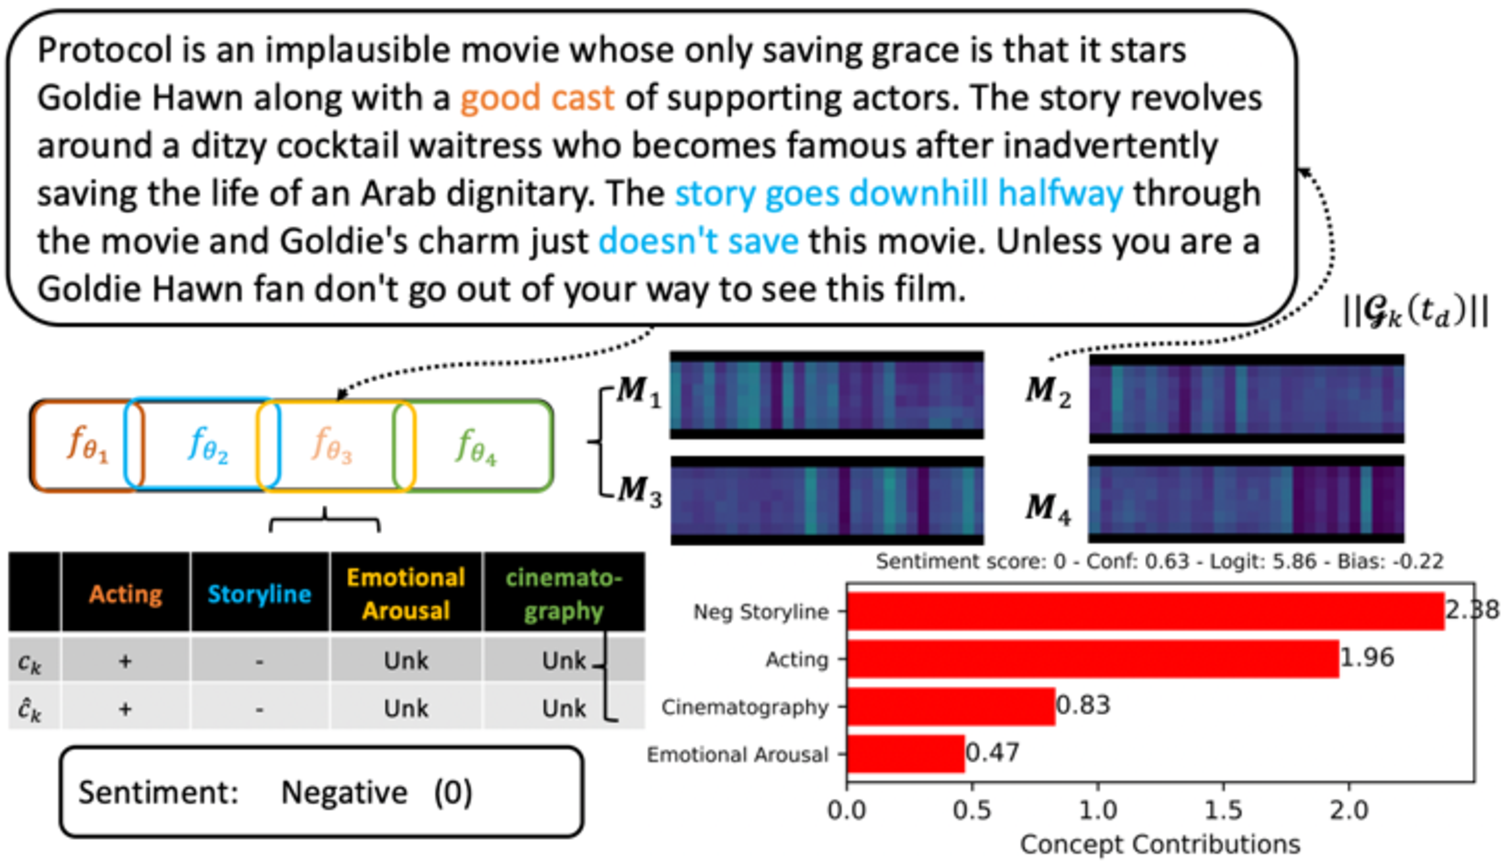
\includegraphics[width=\linewidth]{img/example2.pdf}}
  % %removedVspace
  \caption{{The illustration of a decision pathway of an real-world example (\texttt{IMDB-C} dataset) from the SparseCBM framework with BERT as the backbone. The binary weight masks for each concept is represented as a heatmap.}}\label{fig:example2}
  % %removedVspace
\end{figure*}


\end{document}